\setcounter{chapter}{0}
\graphicspath{{/Users/Mike/phdthesis/MY_THESIS}}
\chapter{\label{sec:clas}The \abbr{CLAS6} detector at Thomas Jefferson National Accelerator Facility }

The analysis performed in this work utilizes data collected during a run period from March 2008 - June 2008. The experiment designation was \g12  which was operated in the \abbr{CLAS6} detector\cite{clas} at the Thomas Jefferson National Accelerator Facility (\abbr{TJNAF}\label{abbr:tjnaf}) shown in Fig.~\ref{fig:jlab.aerial}, also known as Jefferson Laboratory (\abbr{JLab}\label{abbr:jlab}). The \abbr{CLAS6} detector is housed in hall \desg{B} at \abbr{JLab}. Continuous Electron Beam Accelerator Facility\cite{cebaf}(\abbr{CEBAF}\label{abbr:cebaf}, Fig.~\ref{fig:jlab.cebaf}) is also housed on the \abbr{JLab} site. \abbr{CEBAF} provides a continuous electron beam to three halls \desg{A}, \desg{B} and \desg{C}. Each hall incorporates a particle detector of different characteristics. For this work the hall \desg{B} will \abbr{CLAS6} detector will be mentioned.

\begin{figure}\begin{center}
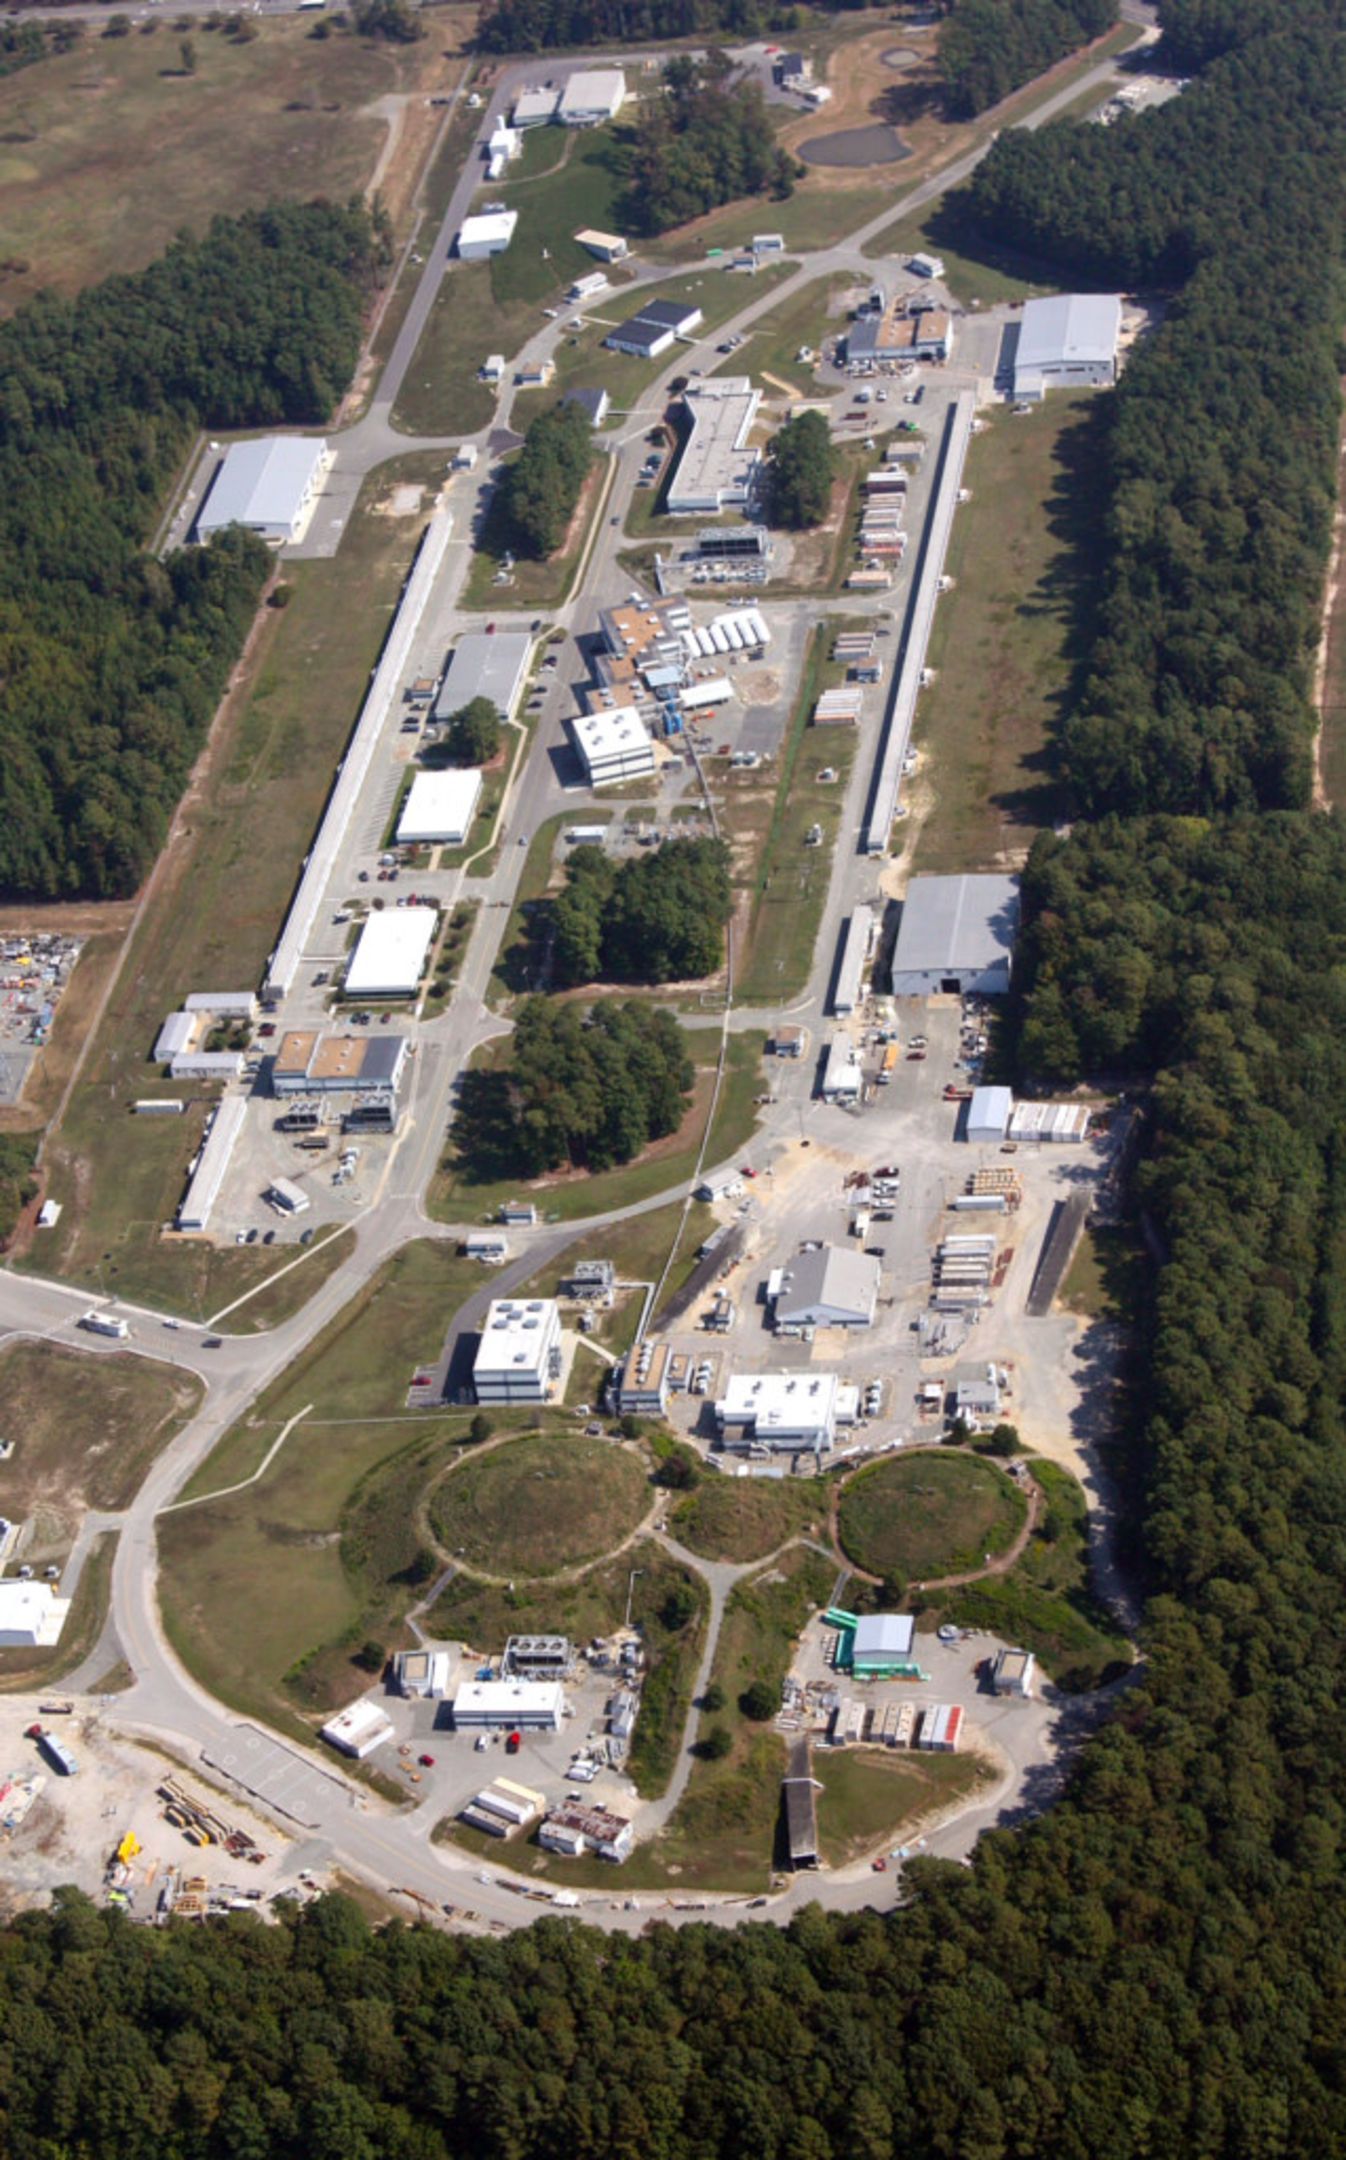
\includegraphics[width=0.6\columnwidth]{\grpath/jlab/jlab_arial_view_II.pdf}
\caption[\abbr{JLab} Aerial View (photograph)]{\label{fig:jlab.aerial}Aerial view of Jefferson Laboratory (\abbr{JLab}) facing east.}
\end{center}\end{figure}

\begin{figure}\begin{center}
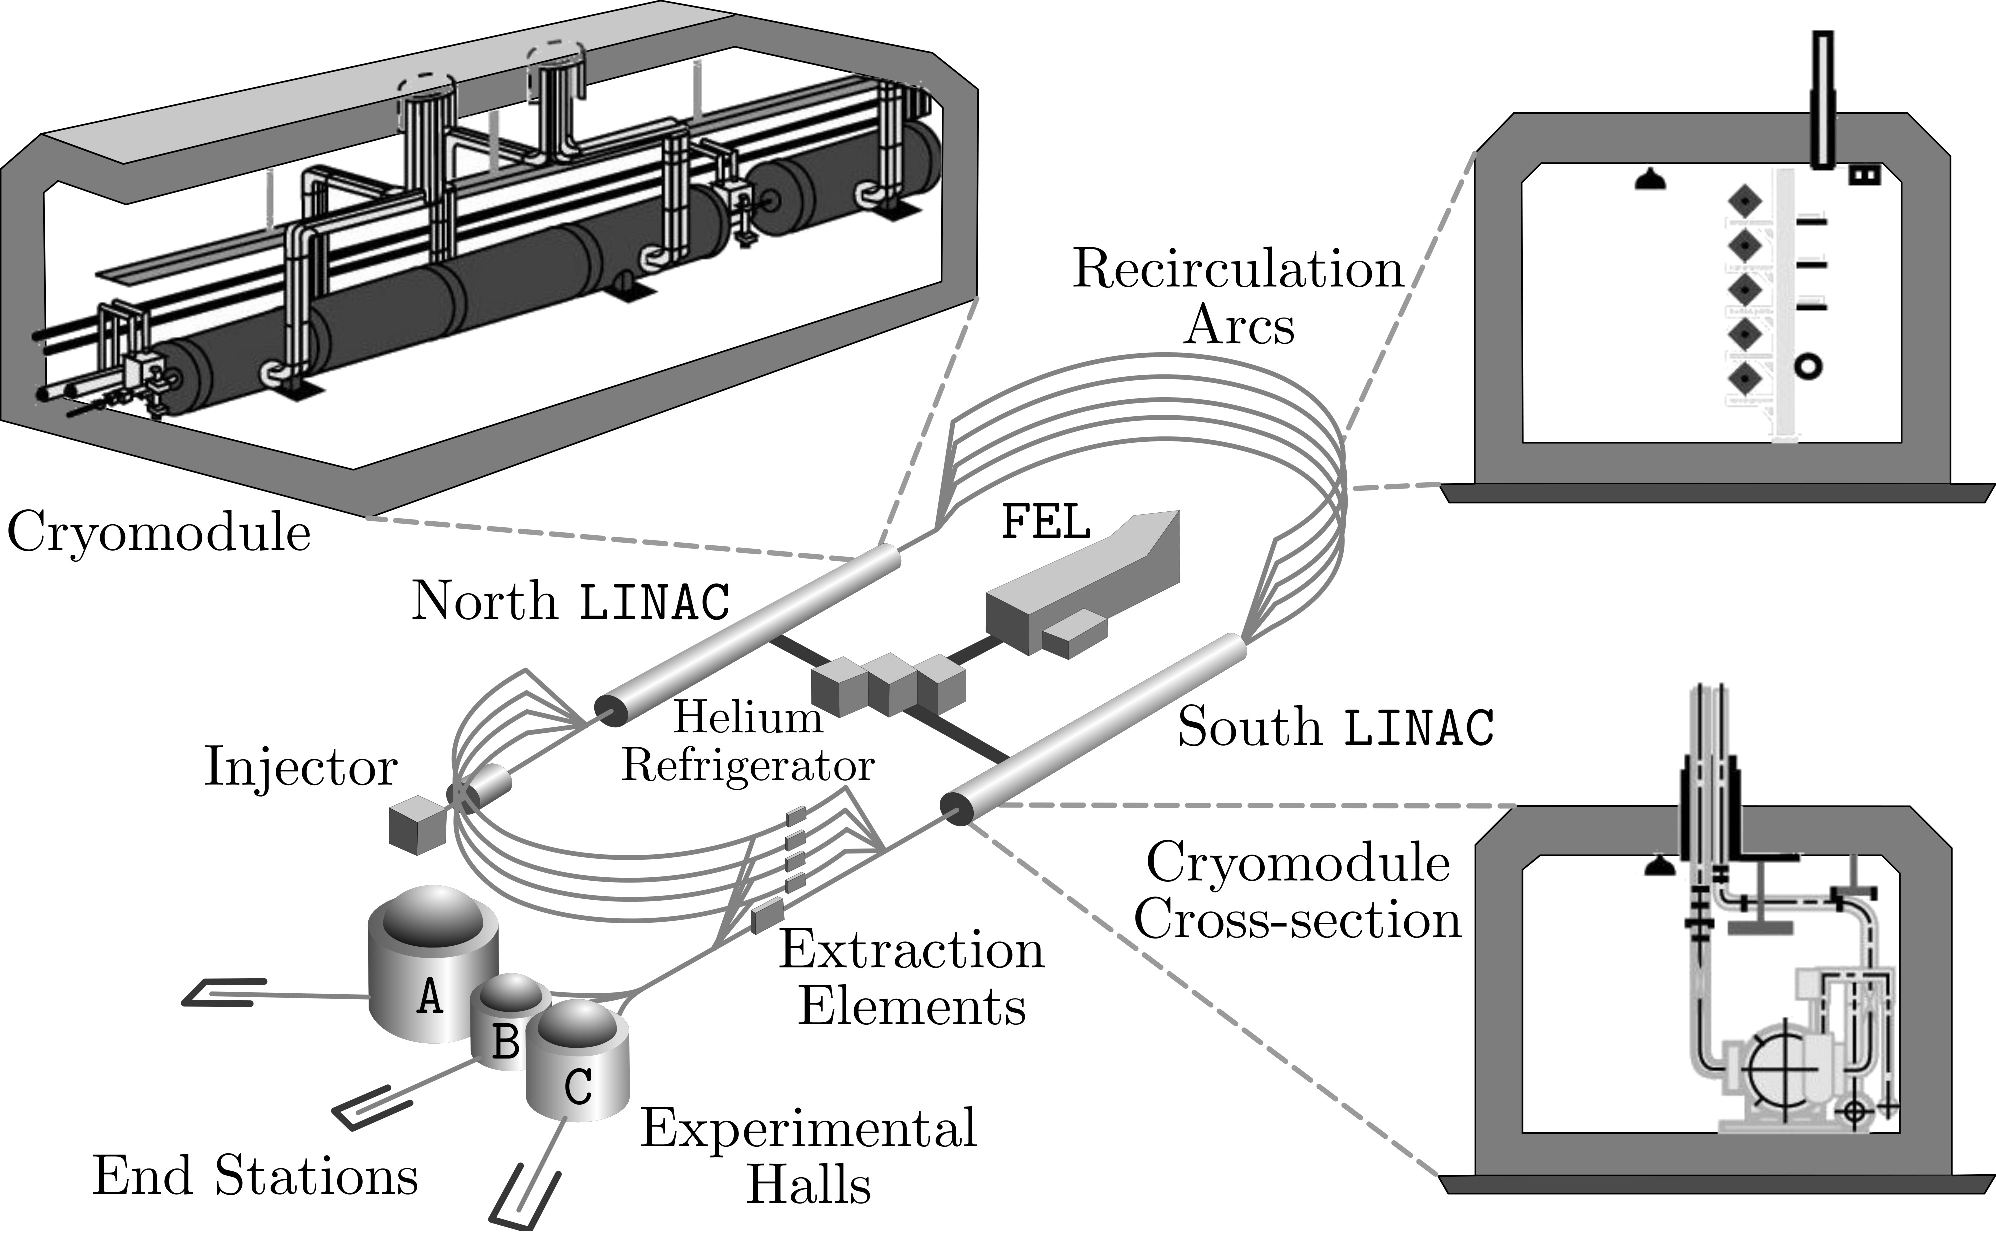
\includegraphics[width=0.9\columnwidth]{\grpath/jlab/cebaf.pdf}
\caption[\abbr{CEBAF} Facility]{\label{fig:jlab.cebaf}The Continuous Electron Beam Accelerator Facility\cite{cebaf} (\abbr{CEBAF}) at Jefferson Laboratory (\abbr{JLab}) showing cross-sections of the linear accelerator (\abbr{LINAC}) halls and the recirculation arcs. Also depicted are the Free Electron Laser (\abbr{FEL}\label{abbr:fel}) and the helium refrigerator and distribution facility.}
\end{center}\end{figure}

In Hall \desg{B} of \abbr{JLab}, the \abbr{CEBAF} Large Angle Spectrometer (\abbr{CLAS6}\label{abbr:clas}) is, in essence, a large acceptance multi-wire proportional drift-chamber (\abbr{DC}). The main purpose of the \abbr{DC} in conjunction with the toroidal magnetic field (see Sec.~\ref{sec:clas.dc}) is to measure the momentum of charged final-state particles that leave the target. For the most part, the rest of the \abbr{CLAS6} detector is used to obtain accurate timing and particle identification. In particular, a photon tagger, specific to Hall \desg{B} \emph{photon runs} as discussed in Sec.~\ref{sec:clas.tagr}, is used to measure the energy of photons incident on the target. In addition, there are several beam intensity and dispersion measuring devices used as described in Sec.~\ref{sec:clas.beam}.

The \abbr{CLAS6} detector, shown in Figs.~\ref{fig:hall-b}, \ref{fig:clas} and \ref{fig:clas.ced}, consists of six segments in $\phi$ (angle about the beam line) called \emph{sectors}, each of which cover approximately $\frac{3}{4}\pi$~radians in $\theta$ (angle from beam line). Each of the six segments consists of a scintillator start counter (\abbr{ST}), three layers of drift chambers (\abbr{DC}), a gas \v{C}erenkov counter (\abbr{CC}), a series of scintillator ``time-of-flight'' (\abbr{TOF}) counters and an electromagnetic calorimeter (\abbr{EC}). There is a toroidal magnetic field concentrated in the middle \abbr{DC} layer which bends charged particles toward or away from the beam line. This field geometry forces the particles to trace a path lying on a plane which allows for a simplied reconstruction algorithm. However, an asymmetry in the acceptance of oppositely charged particles is created.

\begin{figure}\begin{center}
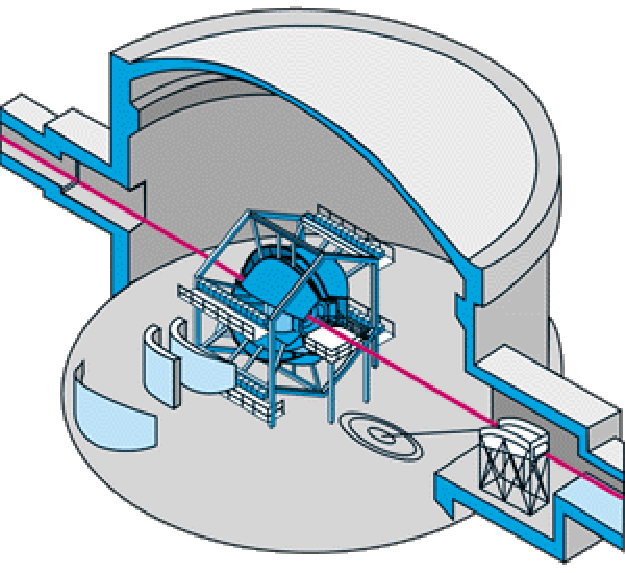
\includegraphics[width=0.5\columnwidth]{\grpath/hall-b/hall-b.pdf}
\caption[Hall \abbr{B}]{\label{fig:hall-b}{\coloronline}Schematic of the \abbr{CLAS6} detector\cite{clas} in Hall \abbr{B} at \abbr{JLab}. The detector is approximately 8~meters in diameter. The beam, indicated by the red line, enters the hall from the lower right and passes through the tagger where the electrons are bent toward the beam dump in the floor and the photons continue to the target.}
\end{center}\end{figure}

\begin{figure}\begin{center}
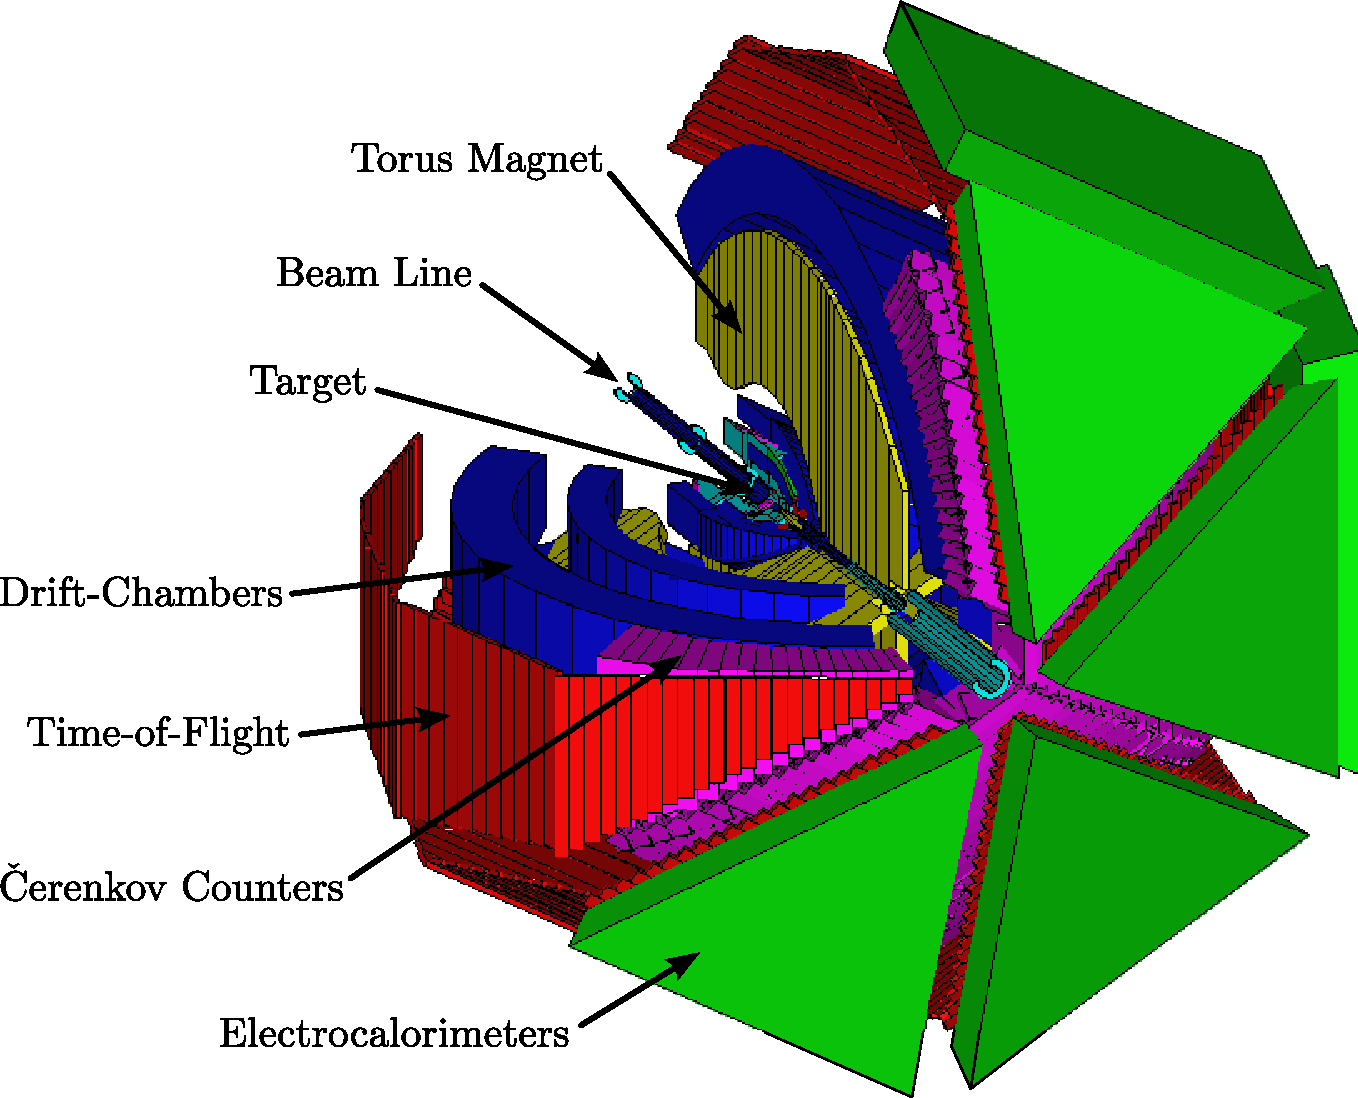
\includegraphics[width=0.8\columnwidth]{\grpath/hall-b/clas_schematic.pdf}
\caption[\abbr{CLAS6} Detector]{\label{fig:clas}{\coloronline}Schematic of the \abbr{CLAS6} detector\cite{clas} with subsystems identified. This view is looking up-stream and the beam enters from the upper left. The detector is approximately 8~meters in diameter.}
\end{center}\end{figure}

\begin{figure}\begin{center}
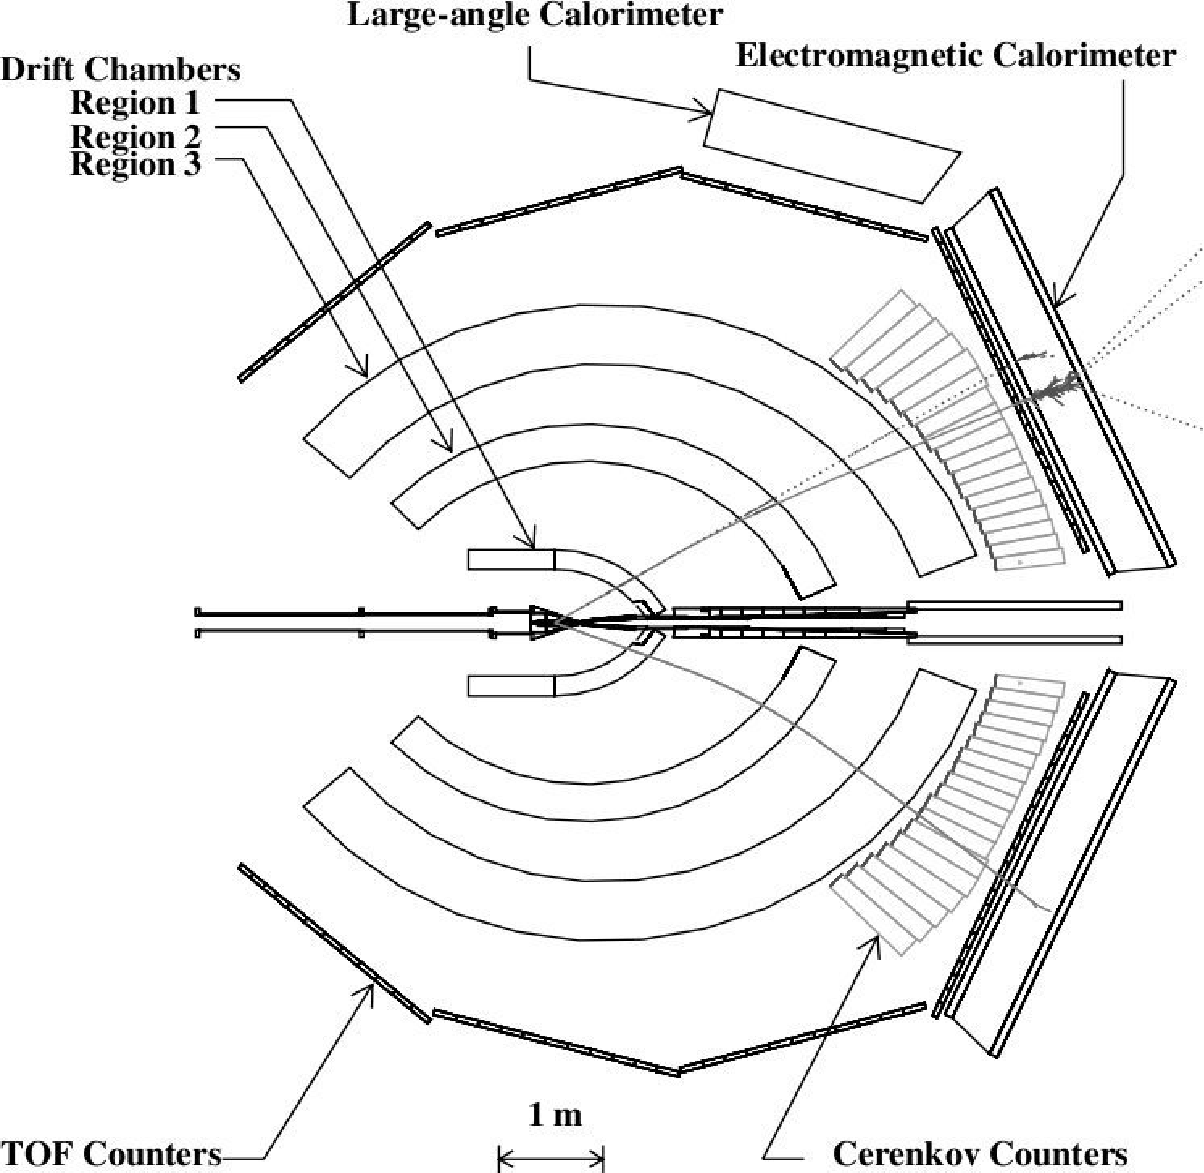
\includegraphics[width=0.6\columnwidth]{\grpath/hall-b/clas_ced.pdf}
\caption[\abbr{CLAS6} Detector Diagram]{\label{fig:clas.ced}A cross section view of the \abbr{CLAS6} detector showing an event with two tracks emanating from the target.}
\end{center}\end{figure}

\section{The \g12 Experiment}\label{sec:clas.g12}

briefly explain the need of \g12

\subsection{\g12 Running Condtions}\label{sec:clas.g12.conditions}

explain \g12, use proposals for this

\subsection{G12 Data Acquisition \& Reconstruction }\label{sec:clas.g12.conditions.data}

Explain g12 data retrieval

\subsection{\g12 Corrections}\label{sec:clas.g12.corrections}

lets write about the beam corrections that were needed because of hysteresis and also the efficiency corrections needed for ''normalization" 
%
%Three \abbr{CLAS} analysis proposals (\abbr{04-005}\cite{clas.proposal.hyclas}, \abbr{04-017}\cite{clas.proposal.superg} and \abbr{08-003}\cite{clas.proposal.pion}) defined the experimental and theoretical basis for the \g12 running period. \label{sec:clas.hyclas}The \abbr{04-005} experiment, \emph{Search for New Forms of Hadronic Matter in Photoproduction}, also called \abbr{HyCLAS}, had a meson spectroscopy focus with multiple charged particle final states such as
%\begin{eqnarray}
%    \gamma \p & \rightarrow & \p \pi^+ \pi^- \pi^0, \\
%    \gamma \p & \rightarrow & \n \pi^+ \pi^+ \pi^-, \\
%    \gamma \p & \rightarrow & \p \Kp \Km \eta, \\
%    \gamma \p & \rightarrow & \n \Kp \Kp \pi^-, \\
%    \gamma \p & \rightarrow & \Delta^{++} \eta \pi^-, \\
%    \gamma \p & \rightarrow & \p \p \bar{\p}.
%\end{eqnarray}
%The physics involved with \abbr{HyCLAS} required the configuration of \abbr{CLAS} to provide the largest acceptance for these multiple particle final states. Phase-space generated events of $\mathrm{\gamma p \rightarrow p \pi^+ \pi^- \pi^0}$ were simulated (see page~30 of \cite{clas.proposal.hyclas}) with the $t$-slope obtained from the \textit{g6c} experiment. The primary requirement for the greatest acceptance of such events was to have the target up-stream (see Sec.~\ref{sec:clas.tgt}) of the normal position at the ``center'' of \abbr{CLAS}. This target placement gave better acceptance for particles close to the beam-line but sacrificed large momentum-transfer events where the final state particles were more than about 70$^\circ$ away from the beam-line.
%
%\label{sec:clas.superg}The \abbr{04-017} experiment, \emph{Study of Pentaquark States in Photoproduction off Protons}, also called \abbr{Super-G}, was founded on a search for the $\Theta^+$ and $\Xi^{--}_{5}$, so-called \emph{penta-quarks}, as well as a study of the ``conventional'' $\Xi$ spectrum (see page~16 of \cite{clas.proposal.superg}.) This analysis is part of the latter topic. The running requirements were similar to that of \abbr{HyCLAS} with the need for a higher energy beam. An examination of the ground state $\Xi^-$ reaction:
%\[
%    \mathrm{\gamma p \rightarrow \Xi^- K^+ K^+},
%\]
%provides a starting point for this analysis. The threshold energy of the incident photon ($E_\gamma$) is given by
%\begin{equation}
%    E_{\gamma} = \frac{m_{\Xi}^2 + 4 m_{\mathrm{K}}^2 + 4 m_{\rule{0pt}{1.4ex}\Xi} m_{\rule{0pt}{1.4ex}\mathrm{K}} - m_{\p}^2}{2 m_{\p}},
%\label{eqn:xi.threshold}
%\end{equation}
%where $m_{\rule{0px}{1.4ex}\Xi}$ is the mass of the $\Xi$, $m_{\rule{0px}{1.4ex}\mathrm{K}}$ is the mass of the K$^{+}$, and $m_{\p}$ is the proton (target particle) mass. For the ground state $\Xi(1320)$ which has a mass of 1.322~GeV, the threshold energy $E_\gamma$ is 2.4 GeV. Since the beam
%(photon) and the target (proton) are both known quantities, we can measure the two kaons and calculate the $\Xi^-$ through ``missing mass'' which is discussed in detail in Chapter~\ref{sec:analysis}. There is a minimum transverse momentum the final state particles must have to be measured by \abbr{CLAS}, otherwise they would travel right down the beam line. Therefore, in order to detect the two kaons with \abbr{CLAS}, a photon energy approximately 0.5~GeV above threshold is required. This corresponds to 2.9~GeV in the reaction for the ground state $\Xi(1320)$.
%
%The third proposal, \abbr{08-003}, titled \emph{The $\gamma \p \rightarrow \pi^+ \n$ Single Charged Pion Photoproduction}, was approved just before the \g12 run period started. This was added onto \g12 as part of the physics to be done with the data collected. It required a single track trigger (see Sec.~\ref{sec:data.trig} on page~\pageref{sec:data.trig}) and lower current. This configuration allowed the data from these special runs to be included in analyses of the ``production'' \g12 data set.
%
%At the beginning of \g12 run, approval came for purchasing gas for the \v{C}erenkov subsystem of \abbr{CLAS}; see Sec.~\ref{sec:clas.cc}. The \v{C}erenkov counters were filled and turned on two weeks into the running period enabling the separation of electons from pions. As a result, a whole new set of leptonic physics became available in what was already a very rich data set.

\section{Electron Accelerator} \label{sec:clas.acc}

The \abbr{CEBAF} electron accelerator is able to deliver a 75\% polarized electron beam of up to approximately 6~GeV to each of the three halls simultaneously. The beam as seen by each hall consists of clusters of electrons separated by approximately 2~ns. Typical intensities for halls \desg{A} and \desg{C} are 10--100~\text{$\mu$} A, however, due to the nature and sensitivity of the \abbr{CLAS} detector, beam currents to hall \desg{B} are typically 10--100~nA.

Using a GaAs photocathode laser driven gun system, a highly polarized electron beam is produced and accelerated through a radio-frequency (\abbr{RF}) chopping system operating at 499~MHz. The three-beam, 1497~MHz ``bunch train'' at 100~keV is then longitudinally compressed and accelerated to just over 1\% of the total machine energy before it is injected into the first main accelerator. This compression results in a beam of 2~ps bunches separated by 668~ps.

The main accelerator consists of a pair of linear accelerators (\abbr{LINAC}s\label{abbr:linac}) which consists of twenty cryomodules each containing eight superconducting niobium cavities as shown in Fig.~\ref{fig:jlab.cavity}. This was the first use of superconducting cavities and marked a major advancement in the field of accelerators. Prior to the \abbr{CEBAF} breakthrough, typical accelerating cavities used non-superconducting metals like copper whose resistivity would cause a build up of heat. The niobium superconducting cavities are kept at 2~Kelvin and are non-resistive, eliminating the heating problems of copper. The significant cooling requirements are satisfied by the Lab's Central Helium Liquefier (\abbr{CHL}\label{abbr:chl}).

\begin{figure}\begin{center} 
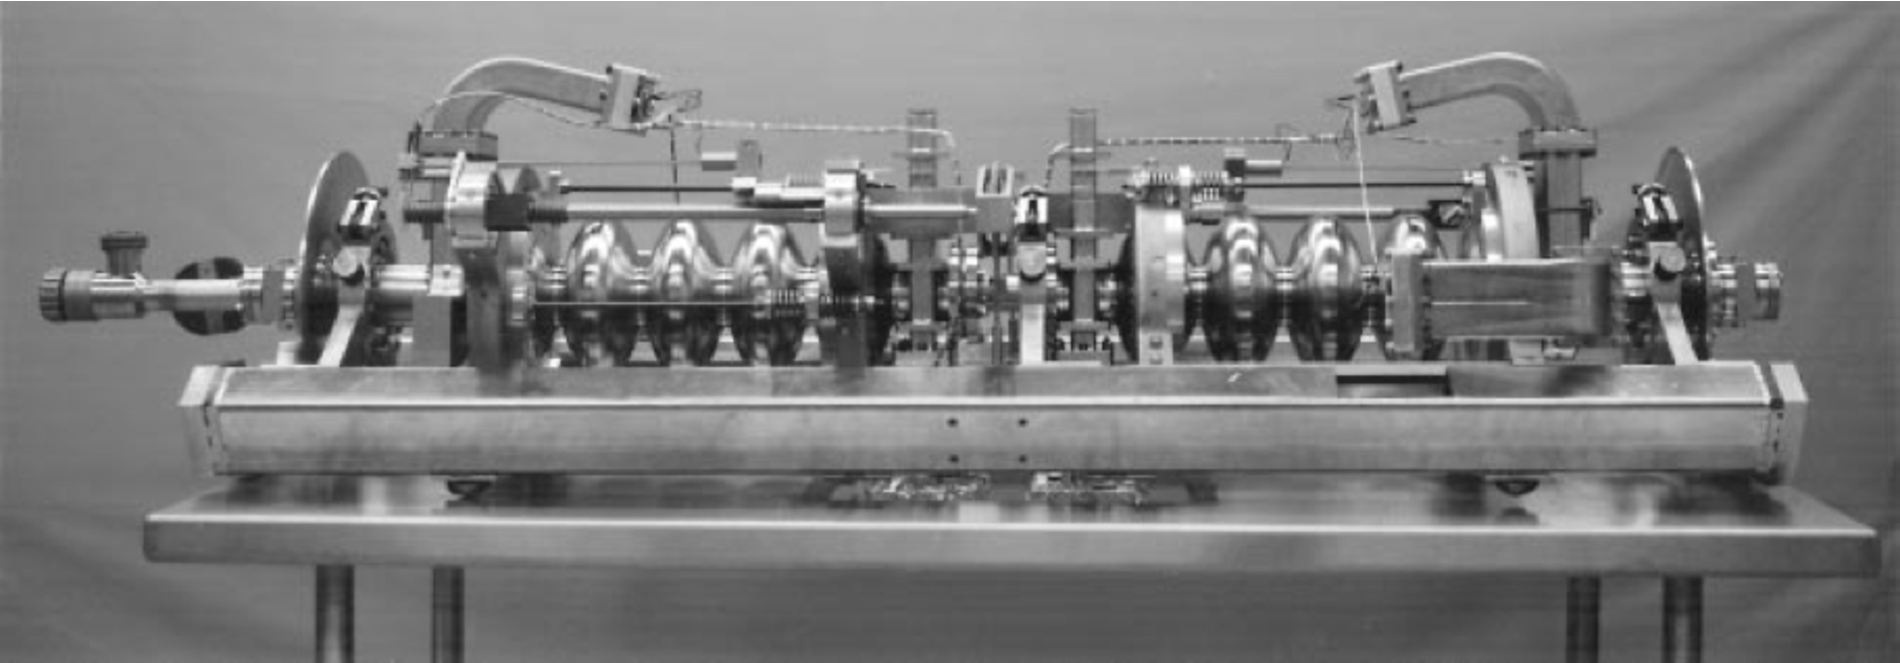
\includegraphics[width=\figwidth]{\grpath/jlab/niobium_cavity_pair.pdf}
\caption[Niobium Cavity Pair (photograph)]{\label{fig:jlab.cavity}A superconducting niobium cavity pair. These devices are tuned for specific energy resonances by mechanically adjusting their lengths on the order of a few micrometers.}
\end{center}\end{figure}

A standing electromagnetic wave is induced inside the niobium cavities as shown in Fig.~\ref{fig:jlab.accel} and the electrons passing through experience a continuous acceleration. Before \abbr{CEBAF}, the copper accelerating cavities used were tuned by adjusting the cooling system. The resistivity of the copper would cause the cavity to heat up and expand and the cooling system would be set so the desired length was obtained. The superconducting niobium cavities on the other hand are non-resistive and do not heat up. Therefore, the cavities are lengthened or shortened mechanically (on the order of a few micrometers) to tune the wavelength and maximize the acceleration of the electrons.

\begin{figure}\begin{center}
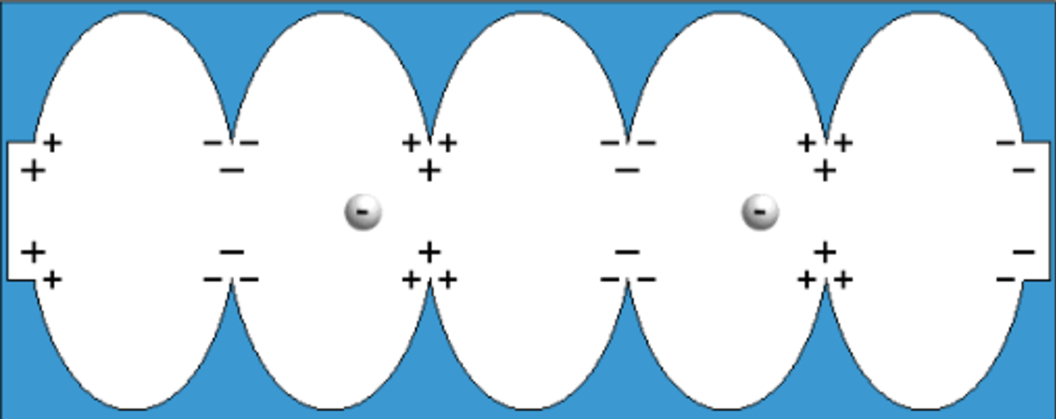
\includegraphics[width=0.8\figwidth]{\grpath/jlab/accelerating_diagram.pdf}
\caption[Accelerating Cavity Diagram]{\label{fig:jlab.accel}As the electron clusters travel through a superconducting niobium cavity, shown in Fig.~\ref{fig:jlab.cavity}, they experience a continuous acceleration due to a standing electromagnetic wave indicated by the positive and negative signs along the inner wall.}
\end{center}\end{figure}

The \abbr{LINAC}s are connected by two sets of 180$^\circ$ magnetic-dipole bending arcs (see Fig.~\ref{fig:jlab.cebaf}) with a radius of 80~meters. The beam is sent through both accelerators and is then \emph{recirculated} up to four more times. Each \abbr{LINAC} is capable of accelerating the beam by up to 600~MeV giving approximately 1.2~GeV per pass. A plan to nearly double the energy of the beam was approved by \abbr{DOE}\label{abbr:doe} and the 12~GeV program started construction on September 15, 2008\cite{jlab.news.cd3, jlab.12gev.starts}.

The beam is selectively extracted using \abbr{RF} cavities tuned to 499~MHz --- the frequency dictated by the manufactured geometry. By slightly accelerating every third bunch, while not disturbing the other two, the electrons are bent out of the recirculating \abbr{LINAC} and sent to one of the halls. Each of the first four passes can be delivered to only one hall at a time, however the fifth (final) pass can be sent to all three halls simultaneously. The 499~MHz extraction creates the final beam as seen by the hall which consists of $\sim2$~ps bunches separated by 2.004~ns. At the time of the \g12 experiment, the accelerator was capable of delivering a maximum electron beam energy of 5.7~GeV. The tagger subsystem (see Sec.~\ref{sec:clas.tagr}) tagged photons of energies up to 95\% of the delivered beam, and therefore the maximum energy photon seen in \g12 was 5.4~GeV.

\FloatBarrier
\section{Beam Positioning}\label{sec:clas.beam}
%\FloatBarrier
There are several beam monitoring stations in Hall \desg{B} before and after the \abbr{CLAS} detector (Fig.~\ref{fig:clas.beam.beforemonitors}) to scan the important details of the electron beam prior to conversion into a photon beam and the details of the photon beam before and after entering the target. Such quantities for the electron beam include position, intensity, dispersion, and current, and for the photon beam include position, dispersion and flux. Most of these monitoring stations are used by the accelerator group.
% to steer the beam to the target as they control all magnets that can substantially move the beam.
\begin{figure}[h!]\begin{center}
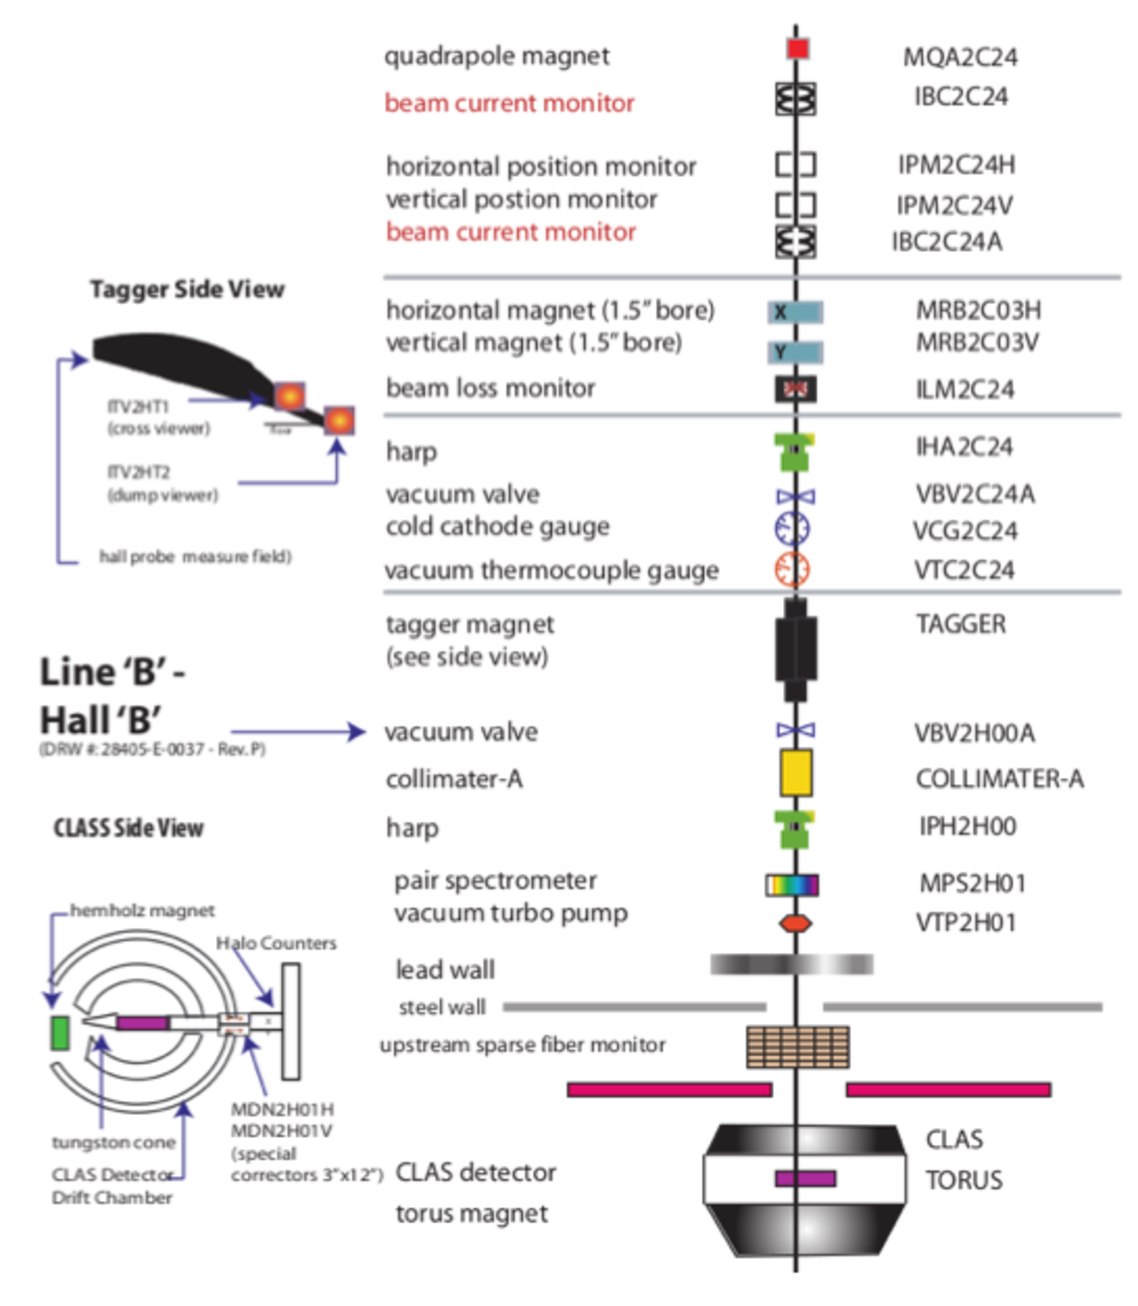
\includegraphics[width=\figwidth, height=1.75\hfigheight]{\grpath/hall-b/beamline_components.pdf}
\caption[Beamline and components of \abbr{CLAS}]{\label{fig:clas.beam.beforemonitors}{\coloronline}Beamline and components of \abbr{CLAS}. Image Source~\cite{cebafflckr}}
\end{center}\end{figure}
There are two types of devices to measure the electron beam position. The first type is represented by two beam position monitors (\abbr{BPM}s\label{abbr:bpm}) placed before the tagger. The position monitors use three radiofrequency cavities to measure the transverse location of the electron beam and its intensity. This information is used as feedback for the steering mechanism. The position monitors are noninvasive and measure at a rate of 1 Hz. 
The second type of device used to measure the beam position is the Harp Beam Profile Monitor, which also measures the electron beam dispersion. The harp devices consist of fine wires (20 and 50~{\um} W and 100~{\um} Fe) that can be passed through the beam at specific orientations and collect scattered electrons with a photomultiplier tube. This procedure measures the horizontal ($x$) and vertical ($y$) profile of the electron beam and is performed after any downtime or change in the beam. The accelerator group adjusts the beam position such that more than 99\% of the electron beam goes through the radiator. Since this process is invasive, it was only done when the drift-chambers and \abbr{DAQ} were turned off. A harp scan measurement for \g12 is shown in Fig.~\ref{fig:clas.beam.harpscan}. The width of the beam was contained within a 200 $\mathrm{\mu}$m diameter.



%\begin{figure}\begin{center}
%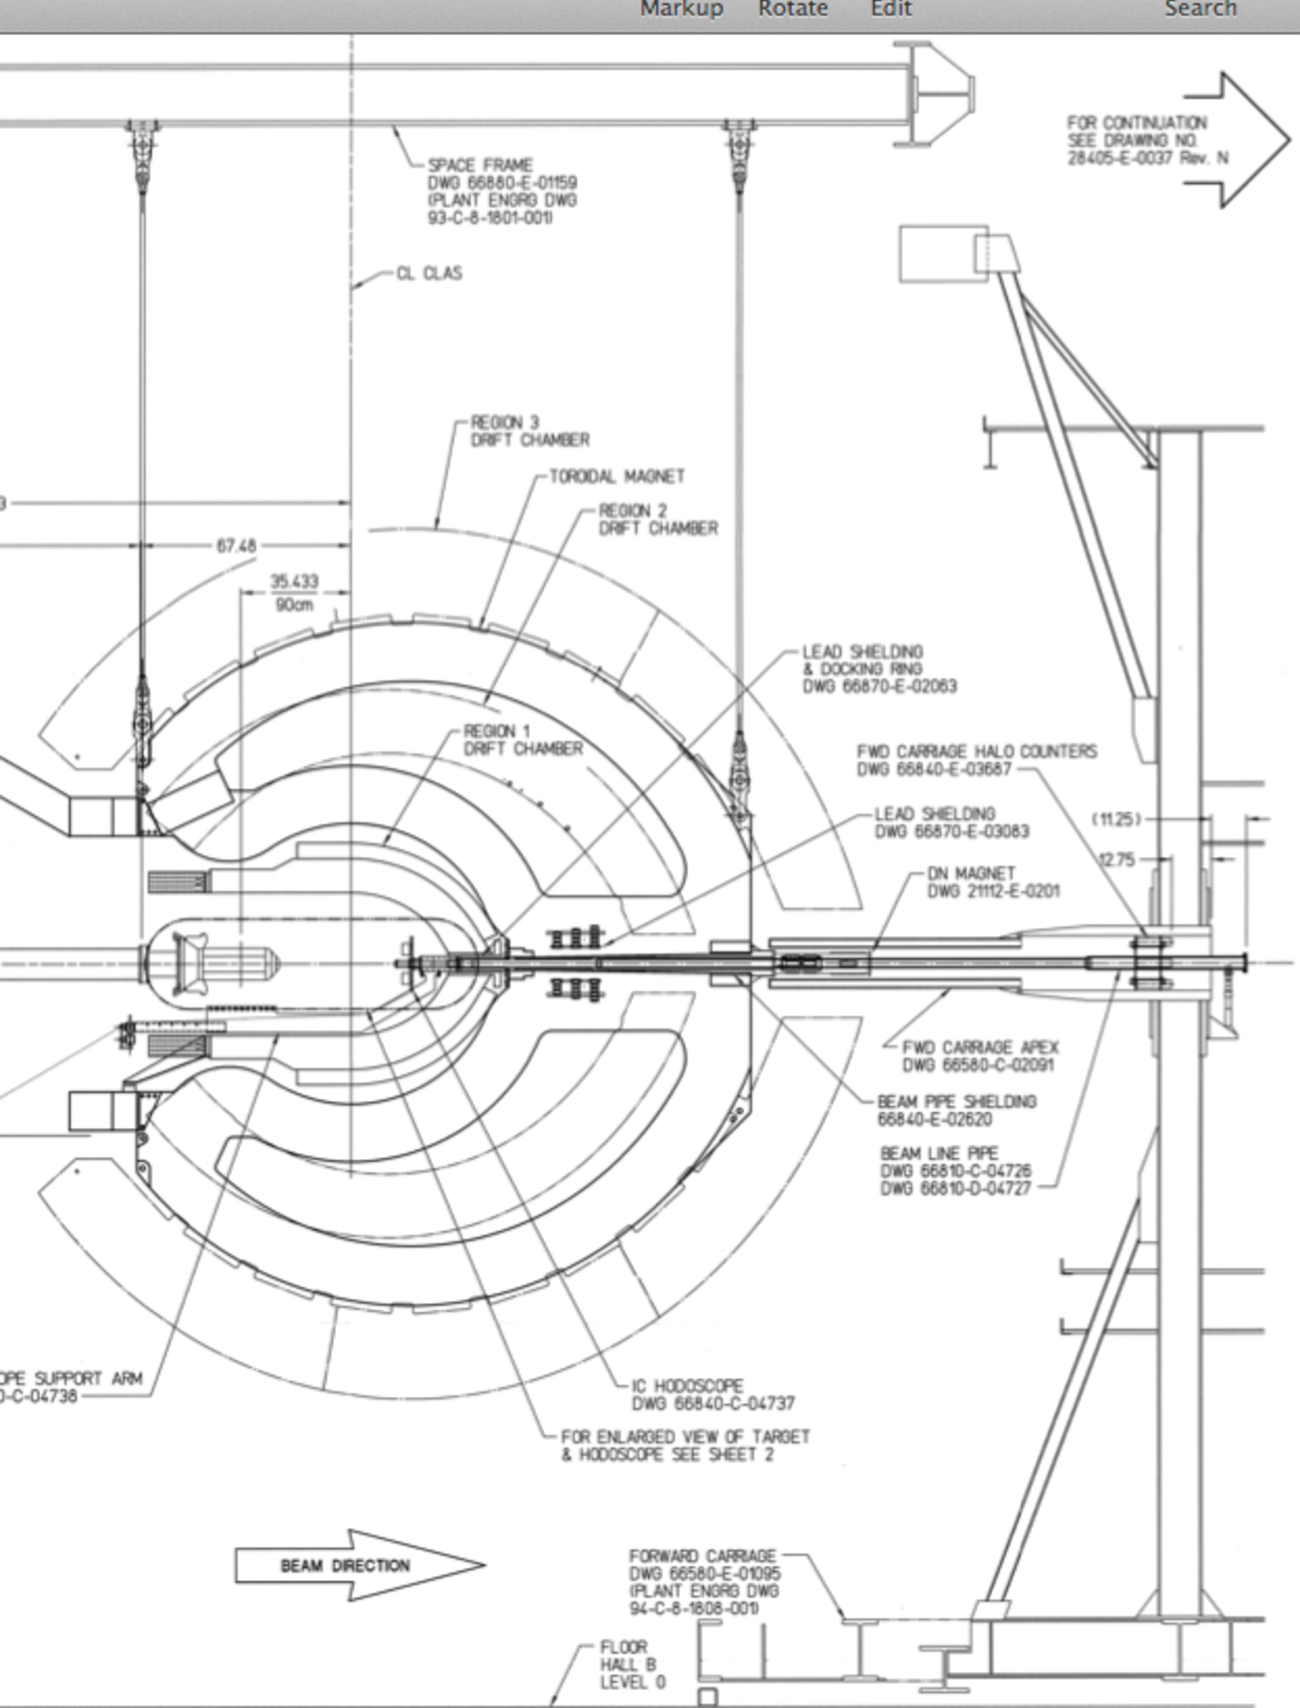
\includegraphics[width=\figwidth,height=\hfigheight]{\grpath/hall-b/G12_afterbeam_blueprint.pdf}
%\caption[Beamline and \abbr{CLAS} components in \g12]{\label{fig:clas.beam.aftermonitors}{\coloronline}Beamline and \abbr{CLAS} components in \g12}
%\end{center}\end{figure}

\begin{figure}\begin{center}
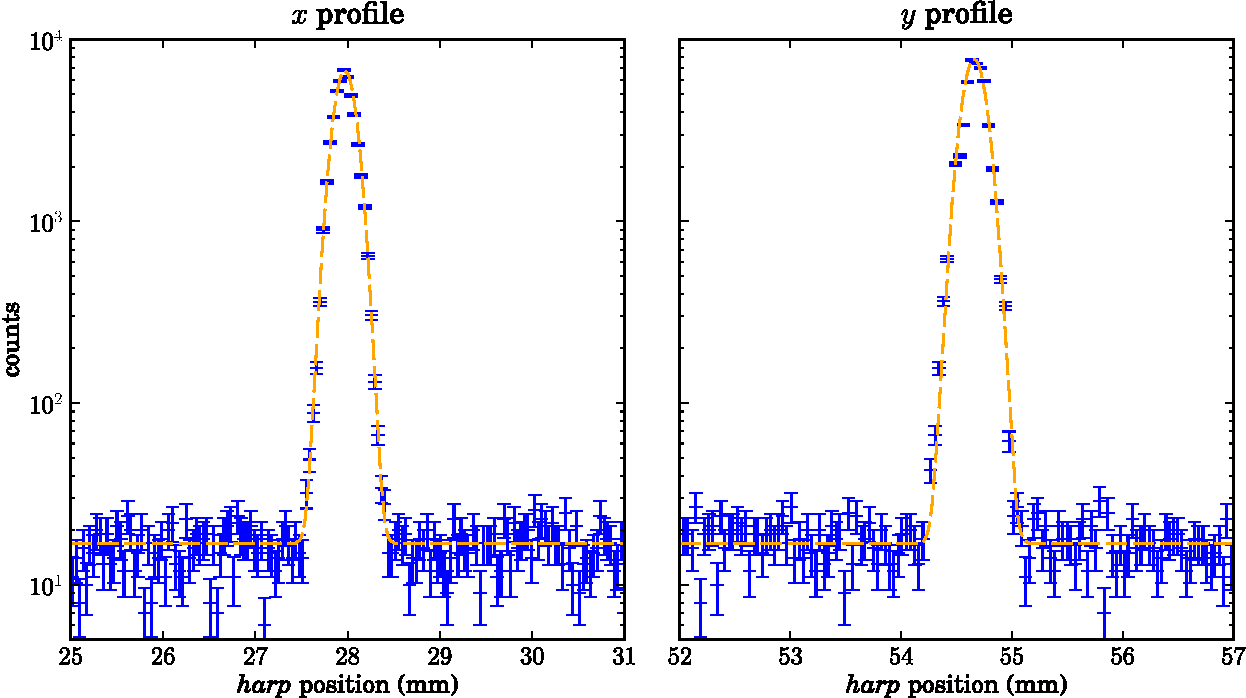
\includegraphics[width=\figwidth,height=\qfigheight]{\grpath/calibration/harpscan.pdf}
\caption[A typical \emph{harp} scan done just prior to run 56426]{\label{fig:clas.beam.harpscan}{\coloronline}A typical \emph{harp} scan done just prior to run 56426. Shown are the $x$ and $y$ profiles of the electron beam just before the tagger. The dashed orange line is a Gaussian fit to the data: $\sigma_x~=~0.115$~mm and $\sigma_y~=~0.105$~mm. Image Source:~\cite{goetz}}
\end{center}\end{figure}

The Total Absorption Shower Counter located downstream of \abbr{CLAS}, measures the photon flux (see Fig.~\ref{fig:clas.beam.afterCLAS}). The \abbr{TASC}, consists of four lead glass blocks of $\sim$ 17 radiation lengths, each coupled to a photo-multiplier tube (\abbr{PMT}\label{abbr:pmt}). The \abbr{TASC} is approximately 100\% efficient at detecting photons at beam currents less than 100~pA\cite{clas.tagger,clas.tagger.calib}. Since \g12 ran with 65~nA current, special low current, 50~pA, normalization runs(see Table~\ref{tab:data.calibruns}) were taken several times throughout \g12. The ratio of electrons detected in the photon tagger (see Sec.~\ref{sec:clas.tagr}) to that of photons detected in the \abbr{TASC} gives the tagging ratio used to calibrate the tagger and measure the flux throughout the entire \g12 run period.
%with hits in the left and right \abbr{TDC} matching in time and a corresponding hit in an E-counter
\begin{figure}[h!]\begin{center}
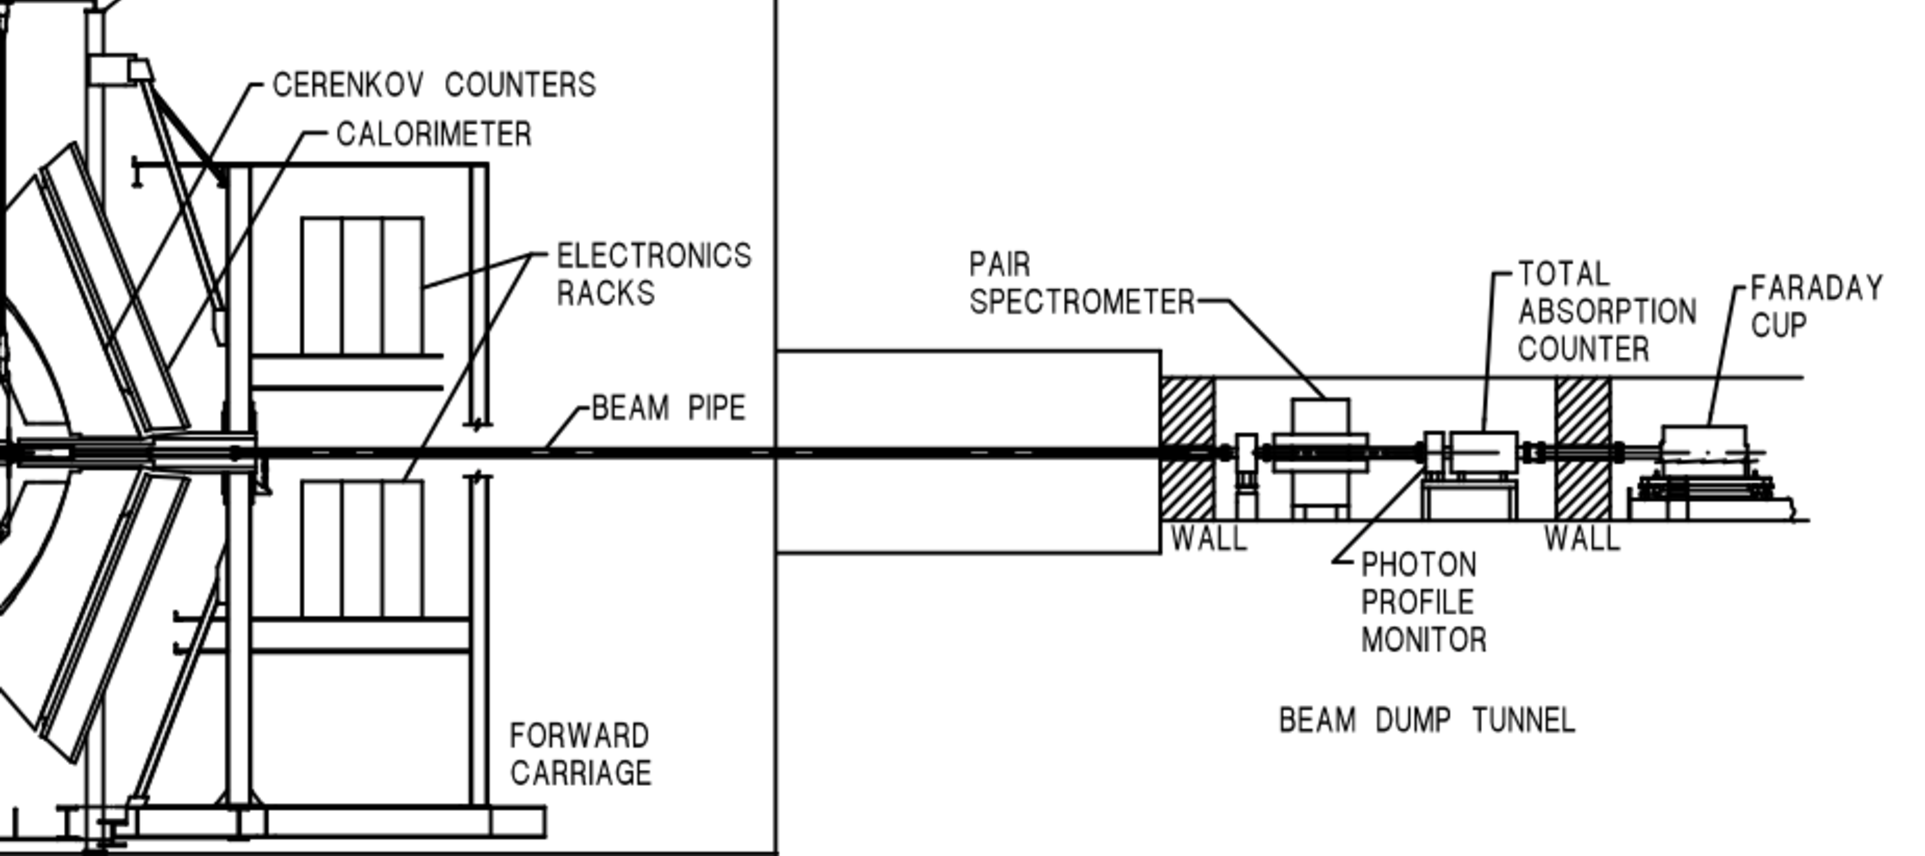
\includegraphics[width=\figwidth,height=0.8\qfigheight]{\grpath/hall-b/TASC_blueprint.pdf}
\caption[Beamline and components after \abbr{CLAS} ]{\label{fig:clas.beam.afterCLAS}{\coloronline}Beamline components in \g12 after \abbr{CLAS}}
\end{center}\end{figure}

\FloatBarrier
\section{\label{sec:clas.tagr}Radiator and Electron Tagger (\abbr{TAG})}

\abbr{CLAS} can use the electron beam as it is delivered from \abbr{CEBAF} by sending it directly to the target. There are a number of experiments which use the electron beam in this fasion. For example, a series of experiments called Deeply Virtual Compton Scattering (\abbr{DVCS}\label{abbr:dvcs}) is currently on-going\cite{avakian2010}, however, the detector is also capable of producing a beam of \emph{real photons} by passing the electrons through a radiator. This causes the electron beam to emit photons via \emph{bremsstrahlung} radiation. The electrons are subsequently bent out of the way by a dipole magnet and the photons continue on to the target. This is known as \emph{photon running} with \abbr{CLAS} and a typical reaction studied looks like
\begin{equation}
	\mathrm{\gamma p \rightarrow p \pi^{+}  \pi^{-}}
\end{equation}

Knowing the incoming electron's energy, the photon's energy can be determined by measuring the momentum of the electron after it has emitted the photon. The electrons are then bent by a dipole magnet and the energy and timing of individual electrons are recorded by the tagger counters\cite{clas.tagger} (\abbr{TAG}) while the photons continue to the target.  In the \g12 experiment, there were usually many ``hits'' in the tagger for each event. Normally, the one associated with the photon that caused the event could be obtained by a timing coincidence with the tracks, though there are cases when this photon is ambiguous as discussed in Sec.~\ref{sec:analysis.beam}.

The \g12 experiment was a \emph{photon run} with an electron beam energy of 5.7~GeV meaning that the tagged photon energy ranged from 1.2 to 5.4~GeV. The radiator used was a gold foil $10^{-4}$~radiation lengths thick. The photons passed through a 6.2~mm diameter collimator 527~cm before they entered the target which had a radius of 2~cm.

\begin{figure}\begin{center}
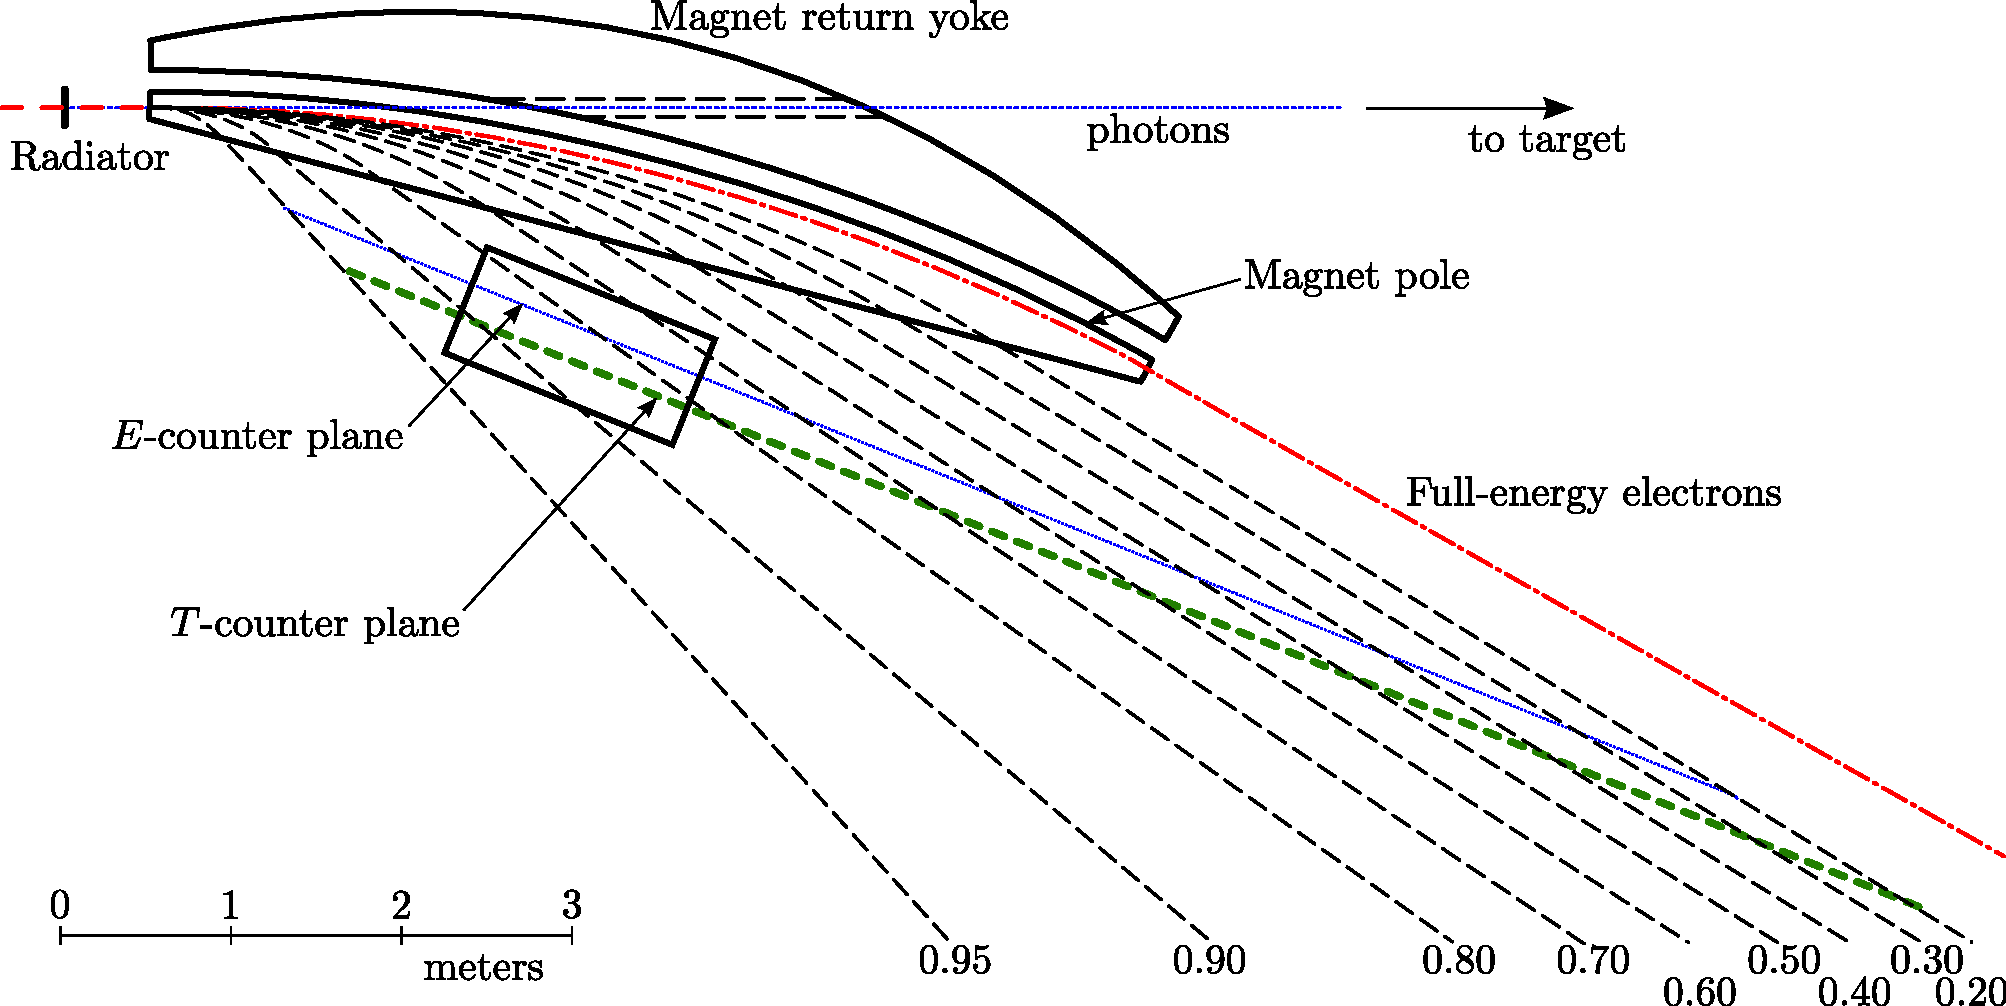
\includegraphics[width=1.1\figwidth]{\grpath/hall-b/tagger_energies.pdf}
\caption[Tagger Schematic - Energies]{\label{fig:jlab.tagr.energies}Scale drawing of the photon tagger system. The electron beam enters from the left and passes through the radiator where a few electrons \emph{bremsstrahl}. The electrons that don't, follow the dash-dot red line to the tagger beam-dump. The electrons that lose energy (black dashed lines) get directed by the dipole magnet to the $E$-counter and $T$-counter planes and the photons continue to the target. The tagging range for the photons is 20\% to 95\% of the beam energy incident on the radiator. The rectangle around the $E$ and $T$-counter planes outlines the expanded view shown in Fig.~\ref{fig:jlab.tagr.paddles}.}
\end{center}\end{figure}

\begin{figure}\begin{center}
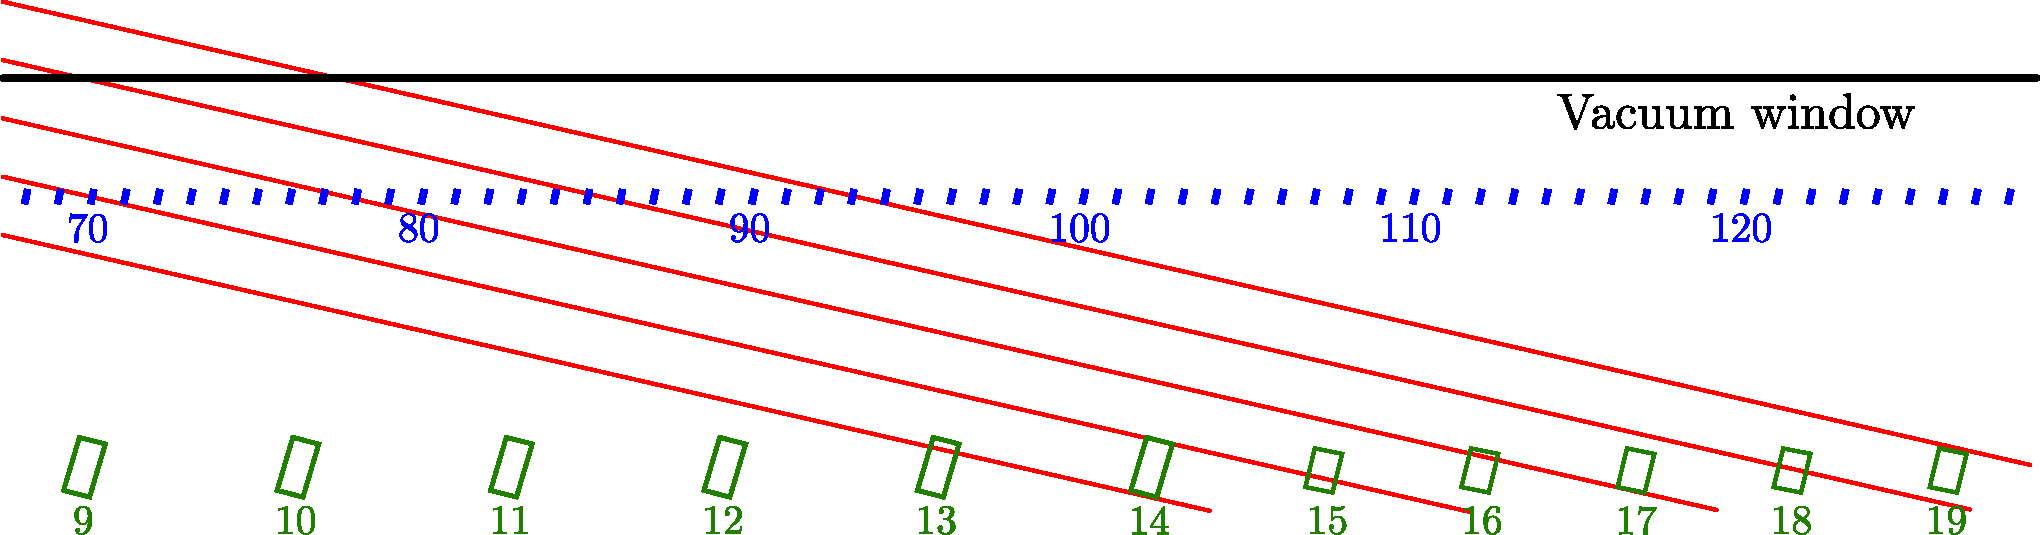
\includegraphics[width=1.1\figwidth]{\grpath/hall-b/tagger_paddles.pdf}
\caption[Tagger Schematic - Paddles]{\label{fig:jlab.tagr.paddles}{\coloronline}Scale drawing of the $E$-counters (upper plane of counters in blue) and the $T$-counters (lower plane of counters in green) showing examples of incident electrons (red lines) entering from the upper left. This view corresponds to the rectangle in Fig.~\ref{fig:jlab.tagr.energies}. Notice how both sets of counters overlap, providing fine segmentation and hermetic coverage. The $T$-counters each consist of two \abbr{PMT}s (\emph{left} and \emph{right}) which are averaged together to obtain the time of the hit. The resolution produced by this setup, crucial for missing mass calculations, is determined by the size and overlap of the $E$-counters as discussed in Sec.~\ref{sec:data.calib.systems}.}
\end{center}\end{figure}

\subsection{Hydrogen Cryotarget}\label{sec:clas.tgt}


The target used by \g12 was conical as shown in Fig.~\ref{fig:clas.targetblueprint}. The target walls were constructed of 0.127~$\mu$m thick Kapton. It is 40~cm in length and 2~cm in radius. The incident photon beam had a radius of 1.5~cm. The target cell design shown in Figs,~\ref{fig:clas.targetblueprint} and~\ref{fig:clas.targetcell} had been used in several experiments and is capable of containing a number of different materials, such as helium, deuterium and hydrogen. For \g12 the target was filled with liquid hydrogen ($\ell$H$_2$). The temperature and pressure of the target was continuously measured and recorded. In Sec~\ref{sec:analysis.target_density}, these measurements will be used to calculate the density of the liquid Hydrogen to determine the target thickness. The target was not polarized.

\begin{figure}[h!]\begin{center}
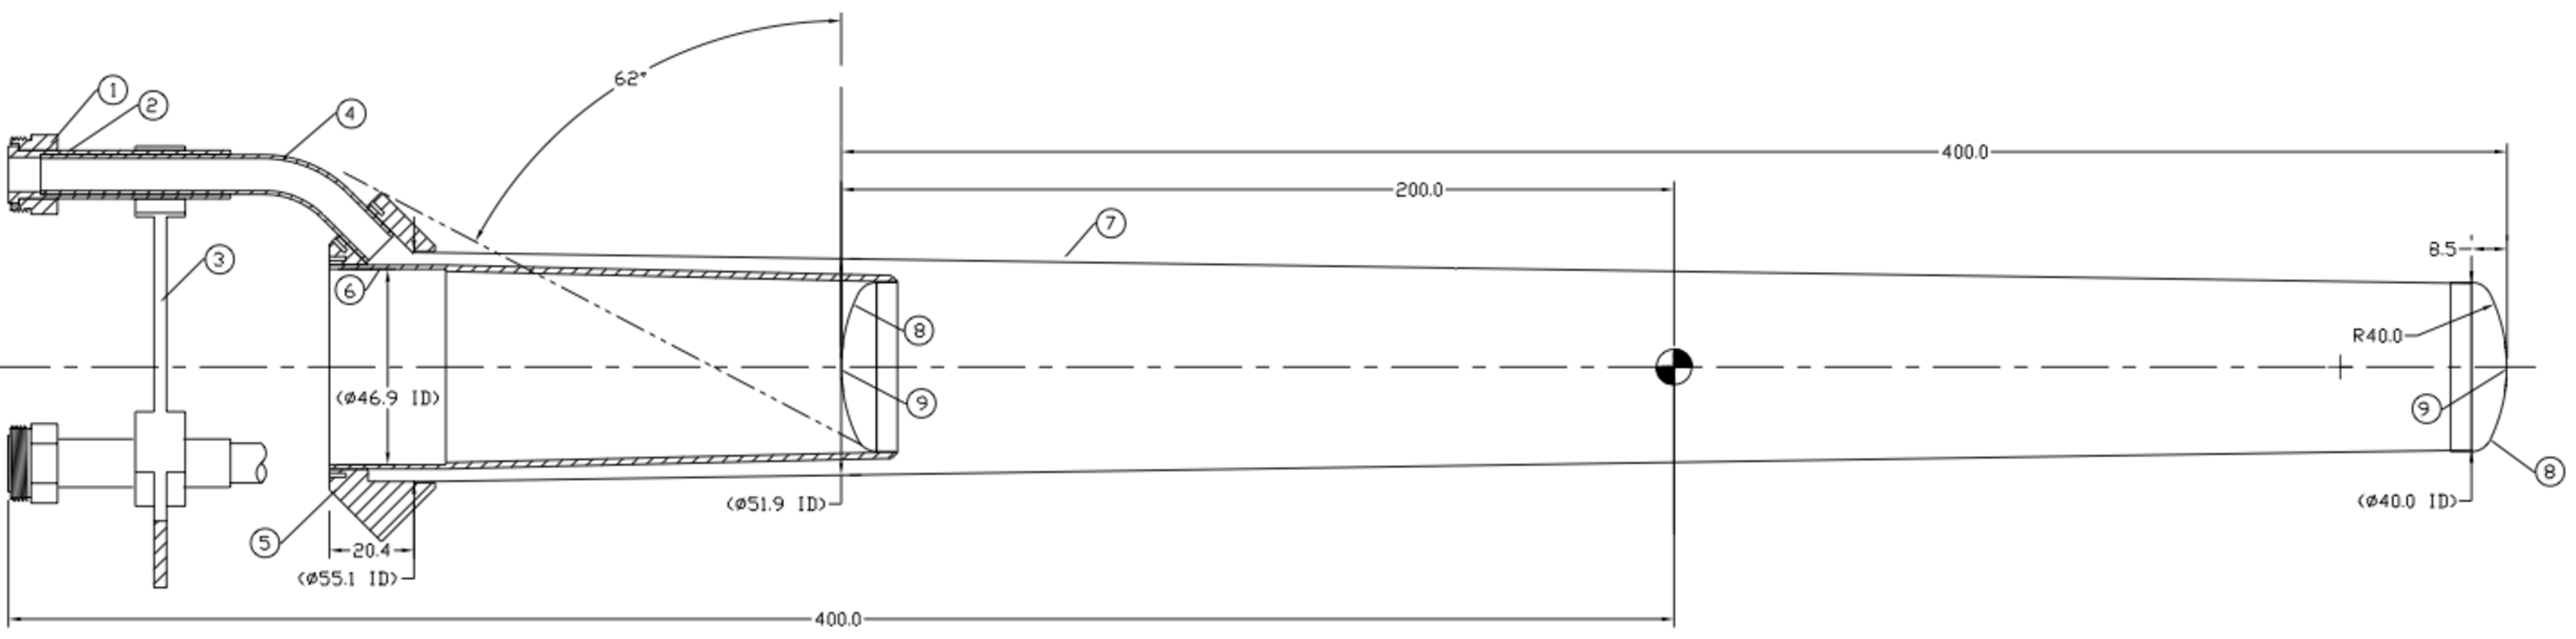
\includegraphics[width=\figwidth,height = \qfigheight]{\grpath/hall-b/g11_target_cell_blueprint.pdf}
\caption[Blueprint schematic of the conical Kapton target cell used for \g12]{\label{fig:clas.targetblueprint}Blueprint schematic of the conical Kapton target cell used for \g12.}
\end{center}\end{figure}

\begin{figure}[h!]\begin{center}
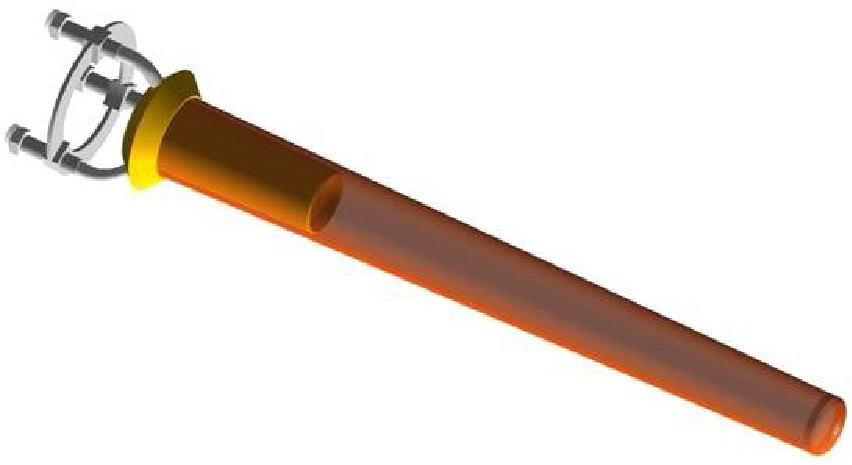
\includegraphics[width=0.6\figwidth]{\grpath/hall-b/g11_target_cell.pdf}
\caption[The 40~cm long conical Kapton target cell used for \g12]{\label{fig:clas.targetcell}The 40~cm long conical Kapton target cell used for \g12.}
\end{center}\end{figure}

%\subsubsection{Target Position for \g12}\label{sec:clas.tgt.position}
The target was located 90~cm upstream of \abbr{CLAS} the center, see Fig.~\ref{fig:clas.ced}.
This increased the forward angle acceptance from 8$^\circ$  to 6$^\circ$. However, this also decreased the large angle acceptance from approximately 140$^\circ$ to 100$^\circ$ in the lab frame.
%This reduction in large angle acceptance sacrificed multi-particle final state events, where the final state particles were more than about 70$^\circ$ away from beamline.
%as well as a reduction in \abbr{DC} resolution. The \abbr{DC} resolution decrease was due to the oblique angle the tracks made with the detector planes.
\FloatBarrier
\section{\label{sec:clas.st}Start Counter (\abbr{ST})}

The first incarnation of \abbr{CLAS} in 1996 had a three segment start counter, each covering two sectors. The data acquisition (\abbr{DAQ}) system at that time had a maximum rate of less than 1~kHz which limited the beam current the detector could handle. Therefore, the hit rate in the start counter was low and the triggering was efficient enough to allow only a few false events. As time went by, the \abbr{DAQ} became more efficient and by 2005 the maximum handling rate was $\sim5$~kHz. This rate was high enough to cause this start counter to act as an open gate in the trigger.

Youri Sharabian, a \abbr{JLab} staff scientist with Hall \desg{B}, designed and built a new 24-segment start counter\cite{clas.st} (\abbr{ST}) in 2006. It was first used with the \emph{g10} experiment\cite{clas.thesis.mckinnon} and it provided better timing and spatial resolution (see Sec.~\ref{sec:data.calib.systems}) as well as the ability to handle much higher beam currents.

The new start counter, shown in Fig.~\ref{fig:clas.st}, consists of 24 scintillation paddles which surrounds the 40~cm target hermetically within the acceptance of the drift-chambers. There are four paddles for each sector and two different paddle shapes. The start counter is capable of approximately 350~ps timing resolution making it useful to identify the hit in the tagger associated with the event. The segmentation allows for event rates that approach the tagger and \abbr{DAQ} limits.

\begin{figure}\begin{center}
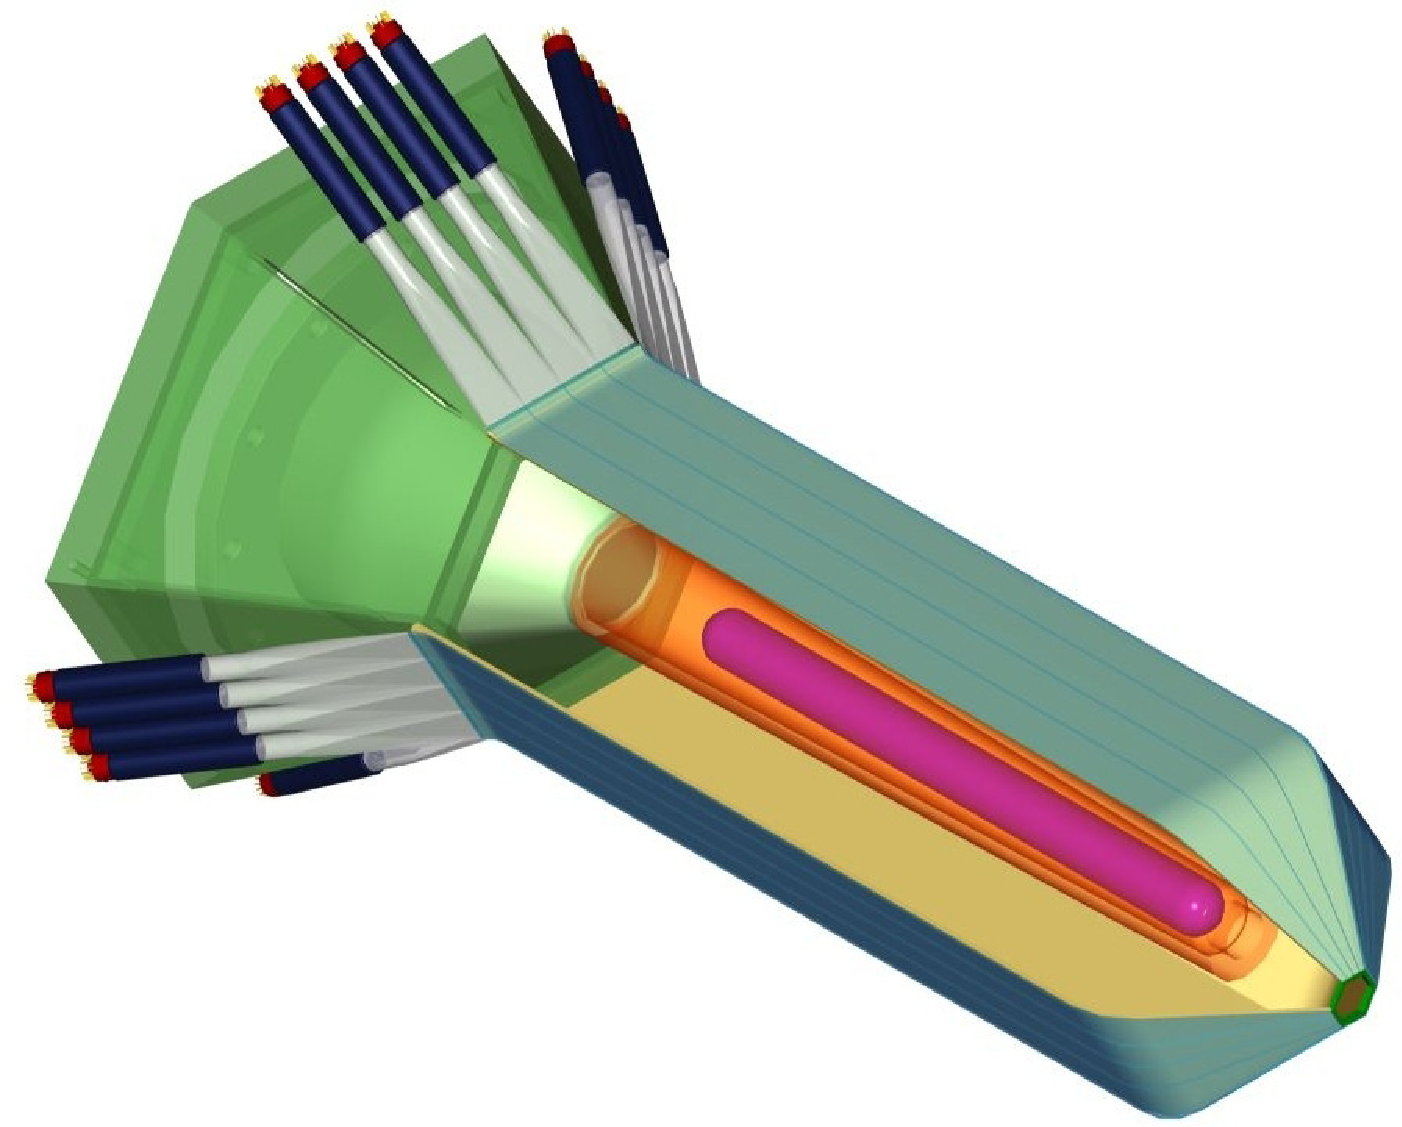
\includegraphics[width=0.8\figwidth]{\grpath/hall-b/start_counter.pdf}
\caption[Start Counter Schematic]{\label{fig:clas.st}{\coloronline}Schematic of the start counter (\abbr{ST}) with the 40~cm long target cell (purple) at the center. The beam enters from the upper left of the figure.}
\end{center}\end{figure}

\begin{figure}\begin{center}
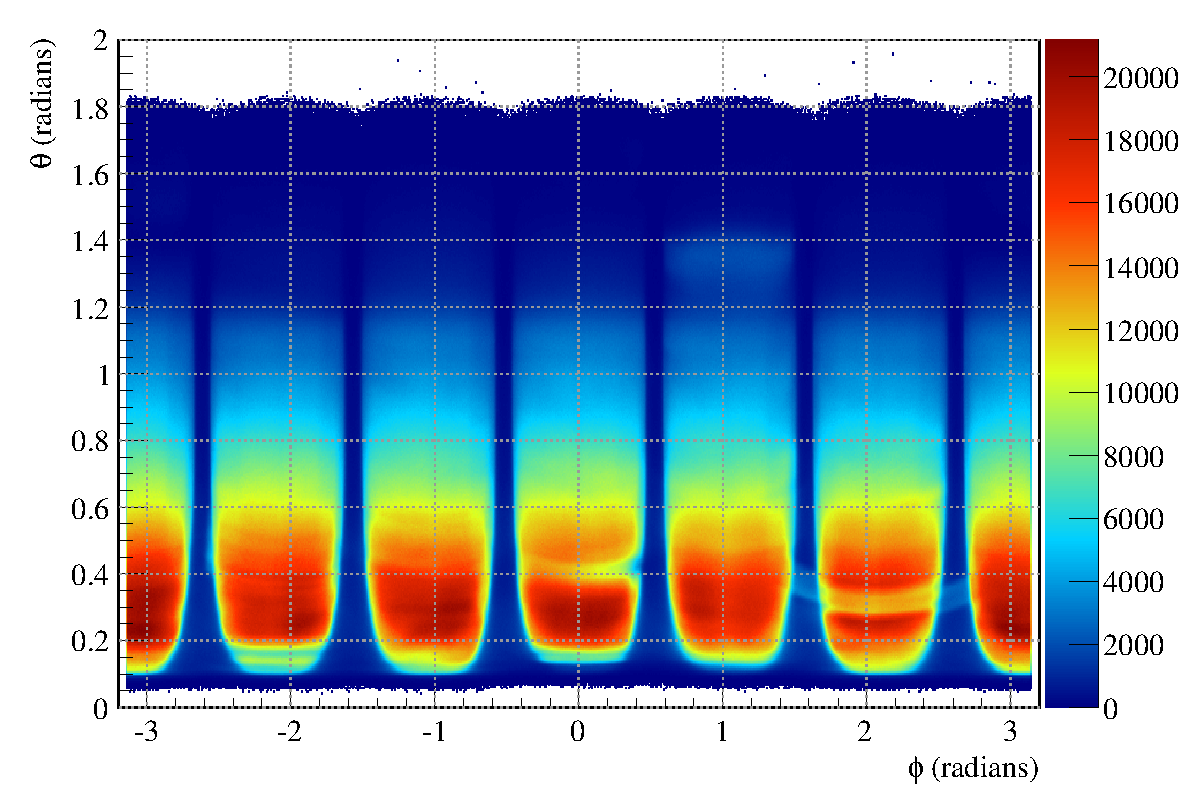
\includegraphics[width=\figwidth]{\grpath/reconstruction/coverage_st.pdf}
\caption[Start Counter Angular Coverage]{\label{fig:clas.st.coverage}{\coloronline}Angular coverage in the lab frame of the tracks that had an associated start counter hit showing that the \abbr{ST} covered the entire \abbr{DC}/\abbr{TOF} acceptance region which is shown in Fig.~\ref{fig:clas.tof.coverage}.}
\end{center}\end{figure}




%\begin{comment}
%
%\subsection{\label{sec:clas.st.eff}Efficiency Analysis}
%
%\todo{NOTE: I'm not sure if I want to keep this section. The numbers quoted are only from memory and are not reliable enough to put here at the moment.}
%
%About a year before \g12, we made some effort to understand the limiting factor on the \abbr{DAQ} rate for \abbr{CLAS}. At the time, it seemed that a start counter segmented in $\theta$ as well as $\phi$ might admit a higher beam current and therefore a higher physics event rate. Using phase-space Monte Carlo of three \emph{prong} events (p $\pi^+$ $\pi^-$) we were able to determine that two tracks will pass through the same \abbr{ST} paddle (in the current 24-paddle configuration) less than 5\% of the time. For topologies requiring four tracks, this increases to about 10\%. This only affects events on the trigger level, and since \g12 used a two-\emph{prong} trigger, the determination was that the 24-segment \abbr{ST} was sufficient. The tracks that use the same start counter hit in the data, since they enter the \abbr{ST} at about the same time, will not be lost during reconstruction.
%
%\begin{figure}\begin{center}
%%\includegraphics[width=0.8\figwidth]{\grpath/reconstruction/start_counter_eff.pdf}
%\caption[Start Counter Efficiency]{\label{fig:clas.st.eff}\todo{This plot must be recreated} Percentage of the track pairs that enter the same \abbr{ST} paddle for topologies increasing in number of particles. The trigger used for \g12 had a two-\emph{prong} configuration and therefore the number events lost at the trigger level was $<1\%$.}
%\end{center}\end{figure}
%
%\end{comment}

%\section{\label{sec:clas.sh}Scintillator Hodoscope (\abbr{SH})}

\todo{NOTE: This section might have to wait (or be cut) untill we actually start using the SH.}

New to \abbr{CLAS}, and installed after the second week of running \g12, was a scintillator hodoscope (\abbr{SH}) placed a few centimeters downstream of the target. This consisted of square ``pixels'' which were read out via silicone photo-counters (\abbr{ScPMC}). This was added in anticipation of the following runs which would use it as a veto counter for the inner calorimeter.

\section{Drift Chambers}\label{sec:clas.dc}

The primary subsystem of the \abbr{CLAS} detector is a collection of multi-wire proportional drift-chambers\cite{clas.dc} (\abbr{DC}) consisting of three layers in each of six sectors as shown in Fig.~\ref{fig:clas}. There is a toroidal magnetic field encompassing the middle layer which causes the charged particles to bend either directly toward or away from the beam-line. The magnetic field at regions 1 and 3 (inner and outer layers respectively) is relatively weak compared to region 2 as shown in Fig.~\ref{fig:clas.dc.torus.mag}. Therefore, the bending of the tracks is concentrated inside region 2 of the \abbr{DC} and the charge and momenta of the particles are determined by measuring the deflection angle of the tracks.

%\begin{figure}\begin{center}
%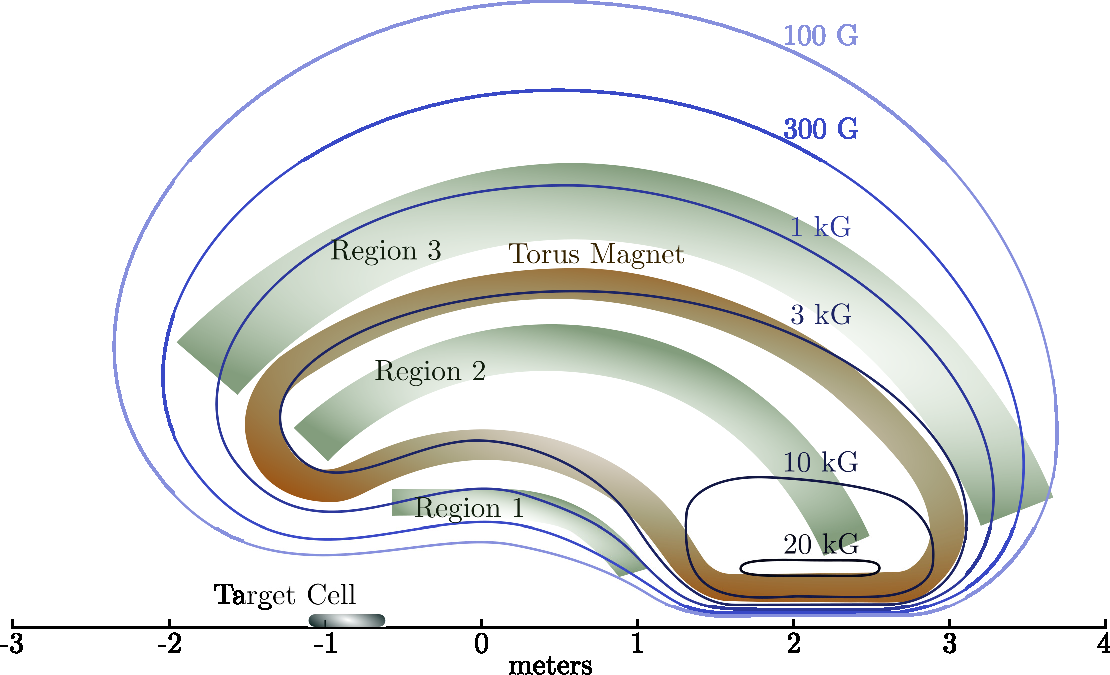
\includegraphics[width=\figwidth]{\figures/hall-b/torus_field_mag.pdf}
%\caption[Magnetic Field Cross-sectional Magnitude]{\label{fig:clas.dc.torus.mag}Cross-section of the toroidal magnetic field at half current (1930~A). For \g12, the direction of the field was into the page and the 40~cm target center was placed at $-90$~cm from the \abbr{CLAS} center. Region 2 of the \abbr{DC} is located inside the region of the coils shown as the kidney shaped loop at about 3~kG.}
%\end{center}\end{figure}

Each region of the \abbr{DC} consists of two \emph{superlayers} which contain six layers of evenly spaced 20~$\mu$m gold-plated tungsten \emph{sense wires} each surrounded by six 140~$\mu$m gold-plated aluminum alloy \emph{field wires}. The very first superlayer (region 1, superlayer 1) has only 4 layers due to space constraints. The field wires were kept at a high negative voltage (approximately $-1.5$~kV) while the sense wires were kept at a moderate positive voltage.

The gas used in the \abbr{DC} is 90\% argon and 10\% carbon-dioxide which is a non-flammable mixture that ionizes easily when charged particles above a certain energy pass through it. The ionized electrons cascade and drift toward the sense wires creating a signal that is amplified and passed through amplifier-discriminator boards (\abbr{ADB}s) and recorded by time-to-digital converters (\abbr{TDC}s). Due to budget considerations, there were no analog-to-digital (\abbr{ADC}) signals recorded from the \abbr{DC}. This could have provided information on the particles' energy loss as it traveled through the chambers, however, energy loss through other systems such as the \abbr{TOF} was available and used in this analysis, as discussed in Chapter~\ref{sec:analysis}.

\section{Cherenkov Counters}\label{sec:clas.cc}


Explain \abbr{CC}
%
%The \emph{gas} \v{C}erenkov counters (\abbr{CC}), indicated in Fig.~\ref{fig:clas}, occupies the space between the drift-chambers and the time-of-flight counters in each of the six sectors. They are divided into 18 segments (shown in Fig.~\ref{fig:clas.cc}) in the polar angle, $\theta$, away from the beam line. These segments are designed to focus \v{C}erenkov-light emitted from particles originating from the center of \abbr{CLAS}. The coverage in $\theta$ is approximately 8$^\circ$ to 45$^\circ$ for tracks originating from the center of \abbr{CLAS}. Because the target was placed 90~cm upstream, the polar coverage was in the range from 6$^\circ$ to 35$^\circ$ in the lab frame.
%
%\begin{figure}\begin{center}
%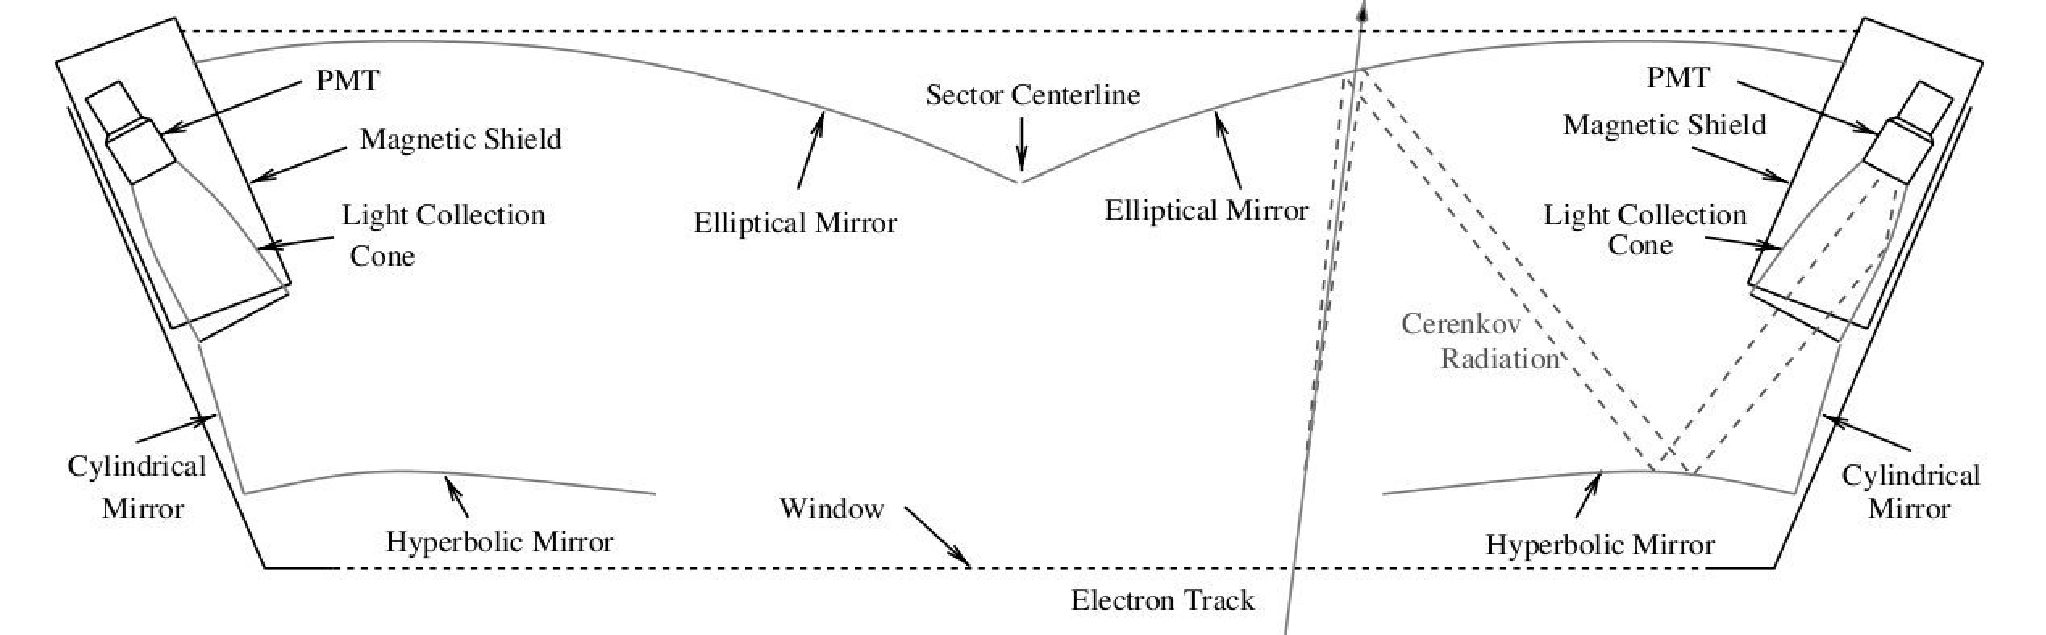
\includegraphics[width=0.9\columnwidth]{\figures/hall-b/cc_diagram.pdf}
%\caption[\v{C}erenkov Detector Segment Diagram]{\label{fig:clas.cc}Diagram of one segment of the \v{C}erenkov counters with an electron entering from the bottom.}
%\end{center}\end{figure}
%
%The gas used in the \abbr{CC} is perfluorobutane (C$_4$F$_{10}$) with an index of refraction of 1.00153. The charged pion threshold for this detector is approximately 2.7~GeV, while the threshold for electrons is 9~MeV. Thresholds for kaons and protons are much higher than the maximum beam energy for \g12 and were therefore not detected in the \abbr{CC}. The detecting efficiency for electrons is $> 97\%$ and this detector enabled the distiction between pions and electrons below approximately 2.5~GeV.
%
%The use of the \abbr{CC} was not included in the original proposals, however a significant drop in price on C$_4$F$_{10}$ just prior to the start of \g12 allowed the gas to be added at the last minute. The price drop was due to the recent availability of another, much cheaper gas that was demonstrated to have the same general properties as C$_4$F$_{10}$.
%
%\begin{figure}\begin{center}
%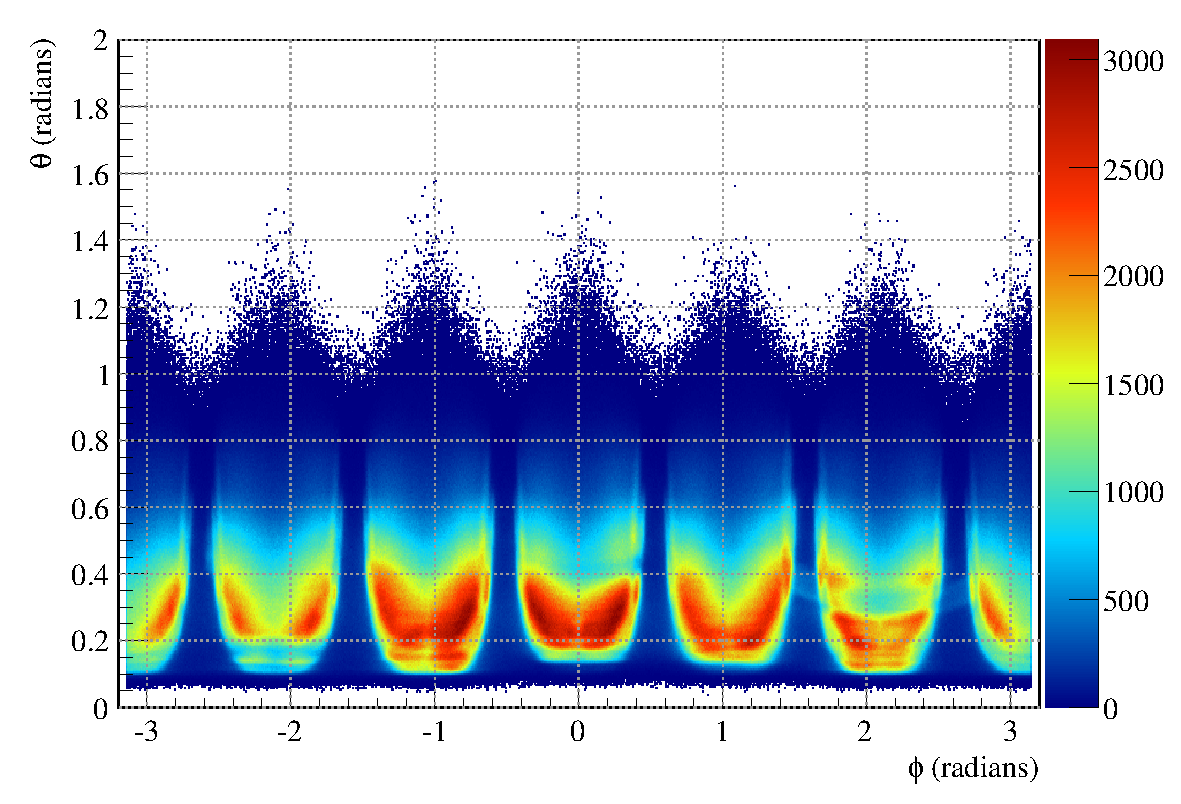
\includegraphics[width=\figwidth]{\figures/reconstruction/coverage_cc.pdf}
%\caption[\v{C}erenkov Counter Angular Coverage]{\label{fig:clas.cc.coverage}{\coloronline}Angular coverage in the lab frame of the tracks that had an associated \v{C}erenkov counter hit.}
%\end{center}\end{figure}

\section{\label{sec:clas.ec}Electromagnetic Calorimeters (\abbr{EC})}

The final layer of the \abbr{CLAS} detector is the electromagnetic calorimeter (\abbr{EC})\cite{clas.ec}, shown in Fig.~\ref{fig:clas}. It consists of alternating layers of lead and scintillator. The overall shape is an equilateral triangle and each layer of scintillator consists of 36 strips as shown in Fig.~\ref{fig:clas.ec}. The \abbr{EC} is divided into an \emph{inner} and \emph{outer} section where the energy deposited from incident tracks is recorded separately.

\begin{figure}\begin{center}

\includegraphics[width=\figwidth]{\figures/hall-b/ec.pdf}
\caption[Electromagnetic Calorimeter Layers]{\label{fig:clas.ec}{\coloronline}Separated view of one sector of the forward electromagnetic calorimeter (\abbr{EC}) showing the three planes ($u$, $v$, $w$) of scintillator-lead pairs which make up one of the 13 \emph{logical} layers.}
\end{center}\end{figure}

The \emph{inner} layer consists of 8 \emph{logical} layers of lead and scintillator while the \emph{outer} layer consists of 5. Each \emph{logical} layer is made of three scintillator-lead layer pairs where the scintillator strips are turned 120$^\circ$ from each other, labeled $u$, $v$ and $w$. There are a total of 39 scintillator-lead layer pairs in each sector of the \abbr{EC}. The angular acceptance of the \abbr{EC} is shown in Fig.~\ref{fig:clas.ec.coverage}. Notice that it covers the entire \v{C}erenkov (Fig.~\ref{fig:clas.cc.coverage}) acceptance region.

\begin{figure}\begin{center}
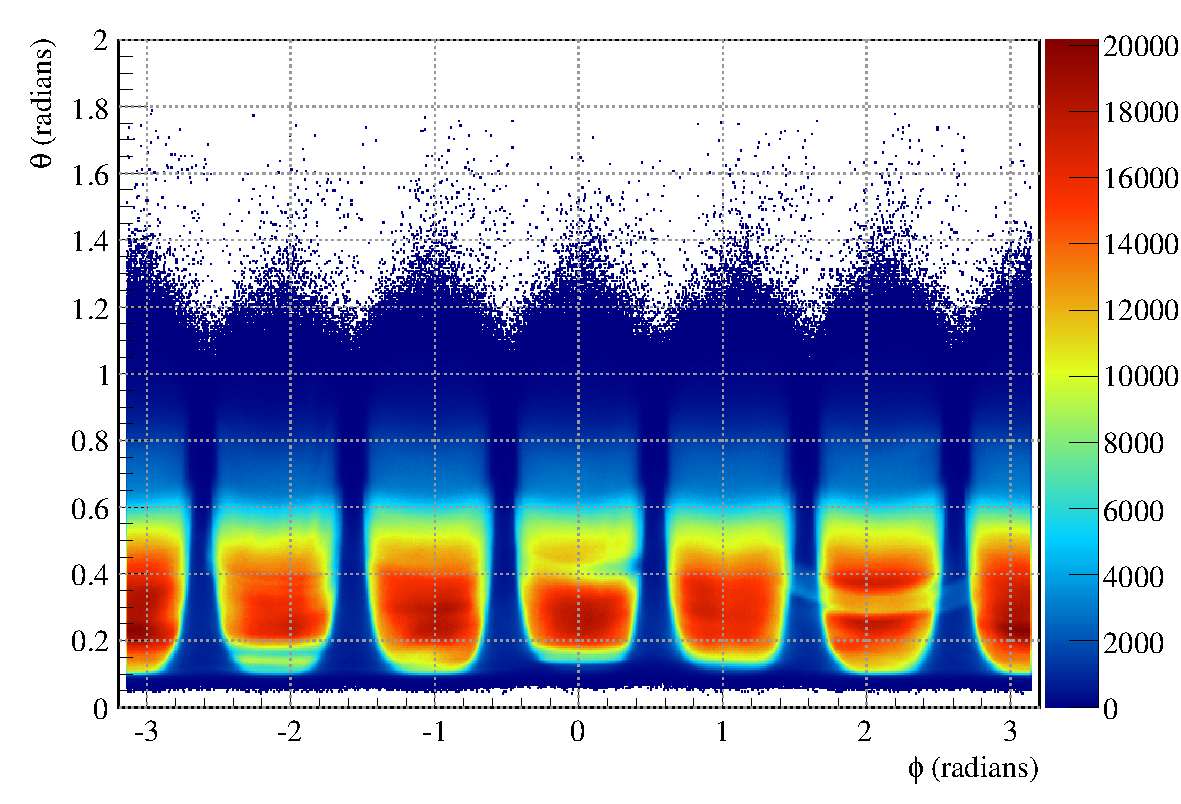
\includegraphics[width=\figwidth]{\figures/reconstruction/coverage_ec.pdf}
\caption[Electromagnetic Calorimeter Angular Coverage]{\label{fig:clas.ec.coverage}{\coloronline}Angular coverage in the lab frame of the tracks that had an associated electromagnetic calorimeter hit.}
\end{center}\end{figure}

The lead to scintillator thickness ratio (0.2) was chosen so one third of the showering particle's energy is deposited into the scintillator. Using the three layers in each \emph{logical} layer to provide pixel-like information, the transverse shower development for a given particle can be determined. The difference in energy deposit between the \emph{inner} and \emph{outer} layers provides separation of electrons from pions in the reconstructed data. For this analysis, the \abbr{EC} was used as a secondary time-of-flight measurement as well as an energy loss determination which provided additional information on particle identification. Furthermore, all final-state photons were identified in the \abbr{EC} by a signature that consisted of a hit only in the first layer of scintillators since the photons are absorbed in the leading sheet of lead.

\section{\label{sec:clas.tof}Time-of-Flight Detectors (\abbr{TOF})}

Accurate measurement of the speed of the final state particles, as discussed in Sec.~\ref{sec:data.calib.systems}, is challenging. Because of their relatively low momentum, typically 1--2~GeV, the particles travel slow enough that the time it takes them to reach the time-of-flight\cite{clas.tof} (\abbr{TOF}) counters is significant. It is thanks to the fine timing resolution of \abbr{CLAS} that enables the \abbr{TOF} to provide the particle identification used in this analysis.

The \abbr{TOF} consists of six outer shells, one of which is shown in Fig.~\ref{fig:clas.tof.paddles}, of 57 scintillator paddles. The paddles are grouped physically into four \emph{panels}. The paddles are all 5.08~cm (2~inches) thick but are of varying lengths and each has a \abbr{PMT} attached to both ends. This provides close to 100\% efficiency of minimum ionizing particles and a timing resolution of 150--200~ps as discussed in Sec.~\ref{sec:data.calib.systems}. The \abbr{TOF} detector was used in the level 1 trigger (see Sec.~\ref{sec:data.trig}) for \g12 to identify ``prongs'' or track candidates. Also, the \abbr{ADC} signals from the \abbr{TOF} were used to measure the energy deposit of the tracks to assist in particle identification in Sec.~\ref{sec:analysis.tofe}.

\begin{figure}\begin{center}
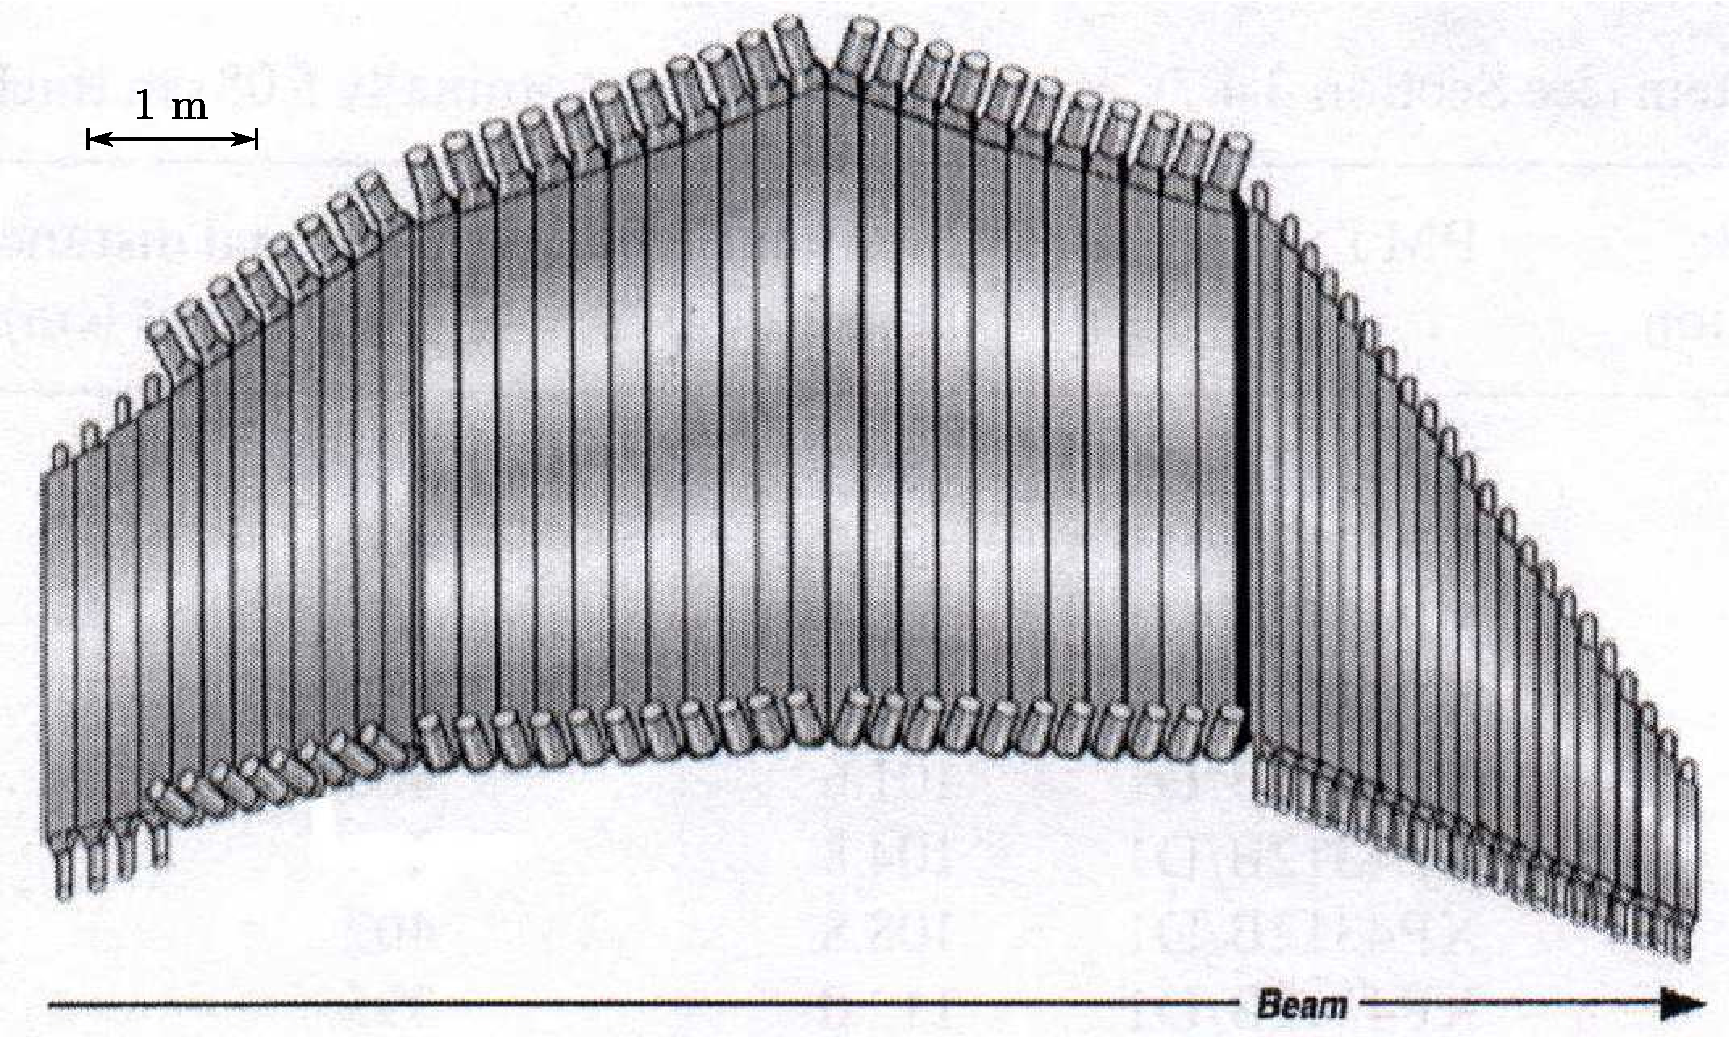
\includegraphics[width=\figwidth]{\figures/hall-b/tof_paddles.pdf}
\caption[Time-of-Flight Paddles]{\label{fig:clas.tof.paddles}Diagram of one sector of the time-of-flight (\abbr{TOF}) paddles. There are 57 scintillator paddles covering the entire acceptance region of the drift-chambers for each sector.}
\end{center}\end{figure}

\begin{figure}\begin{center}
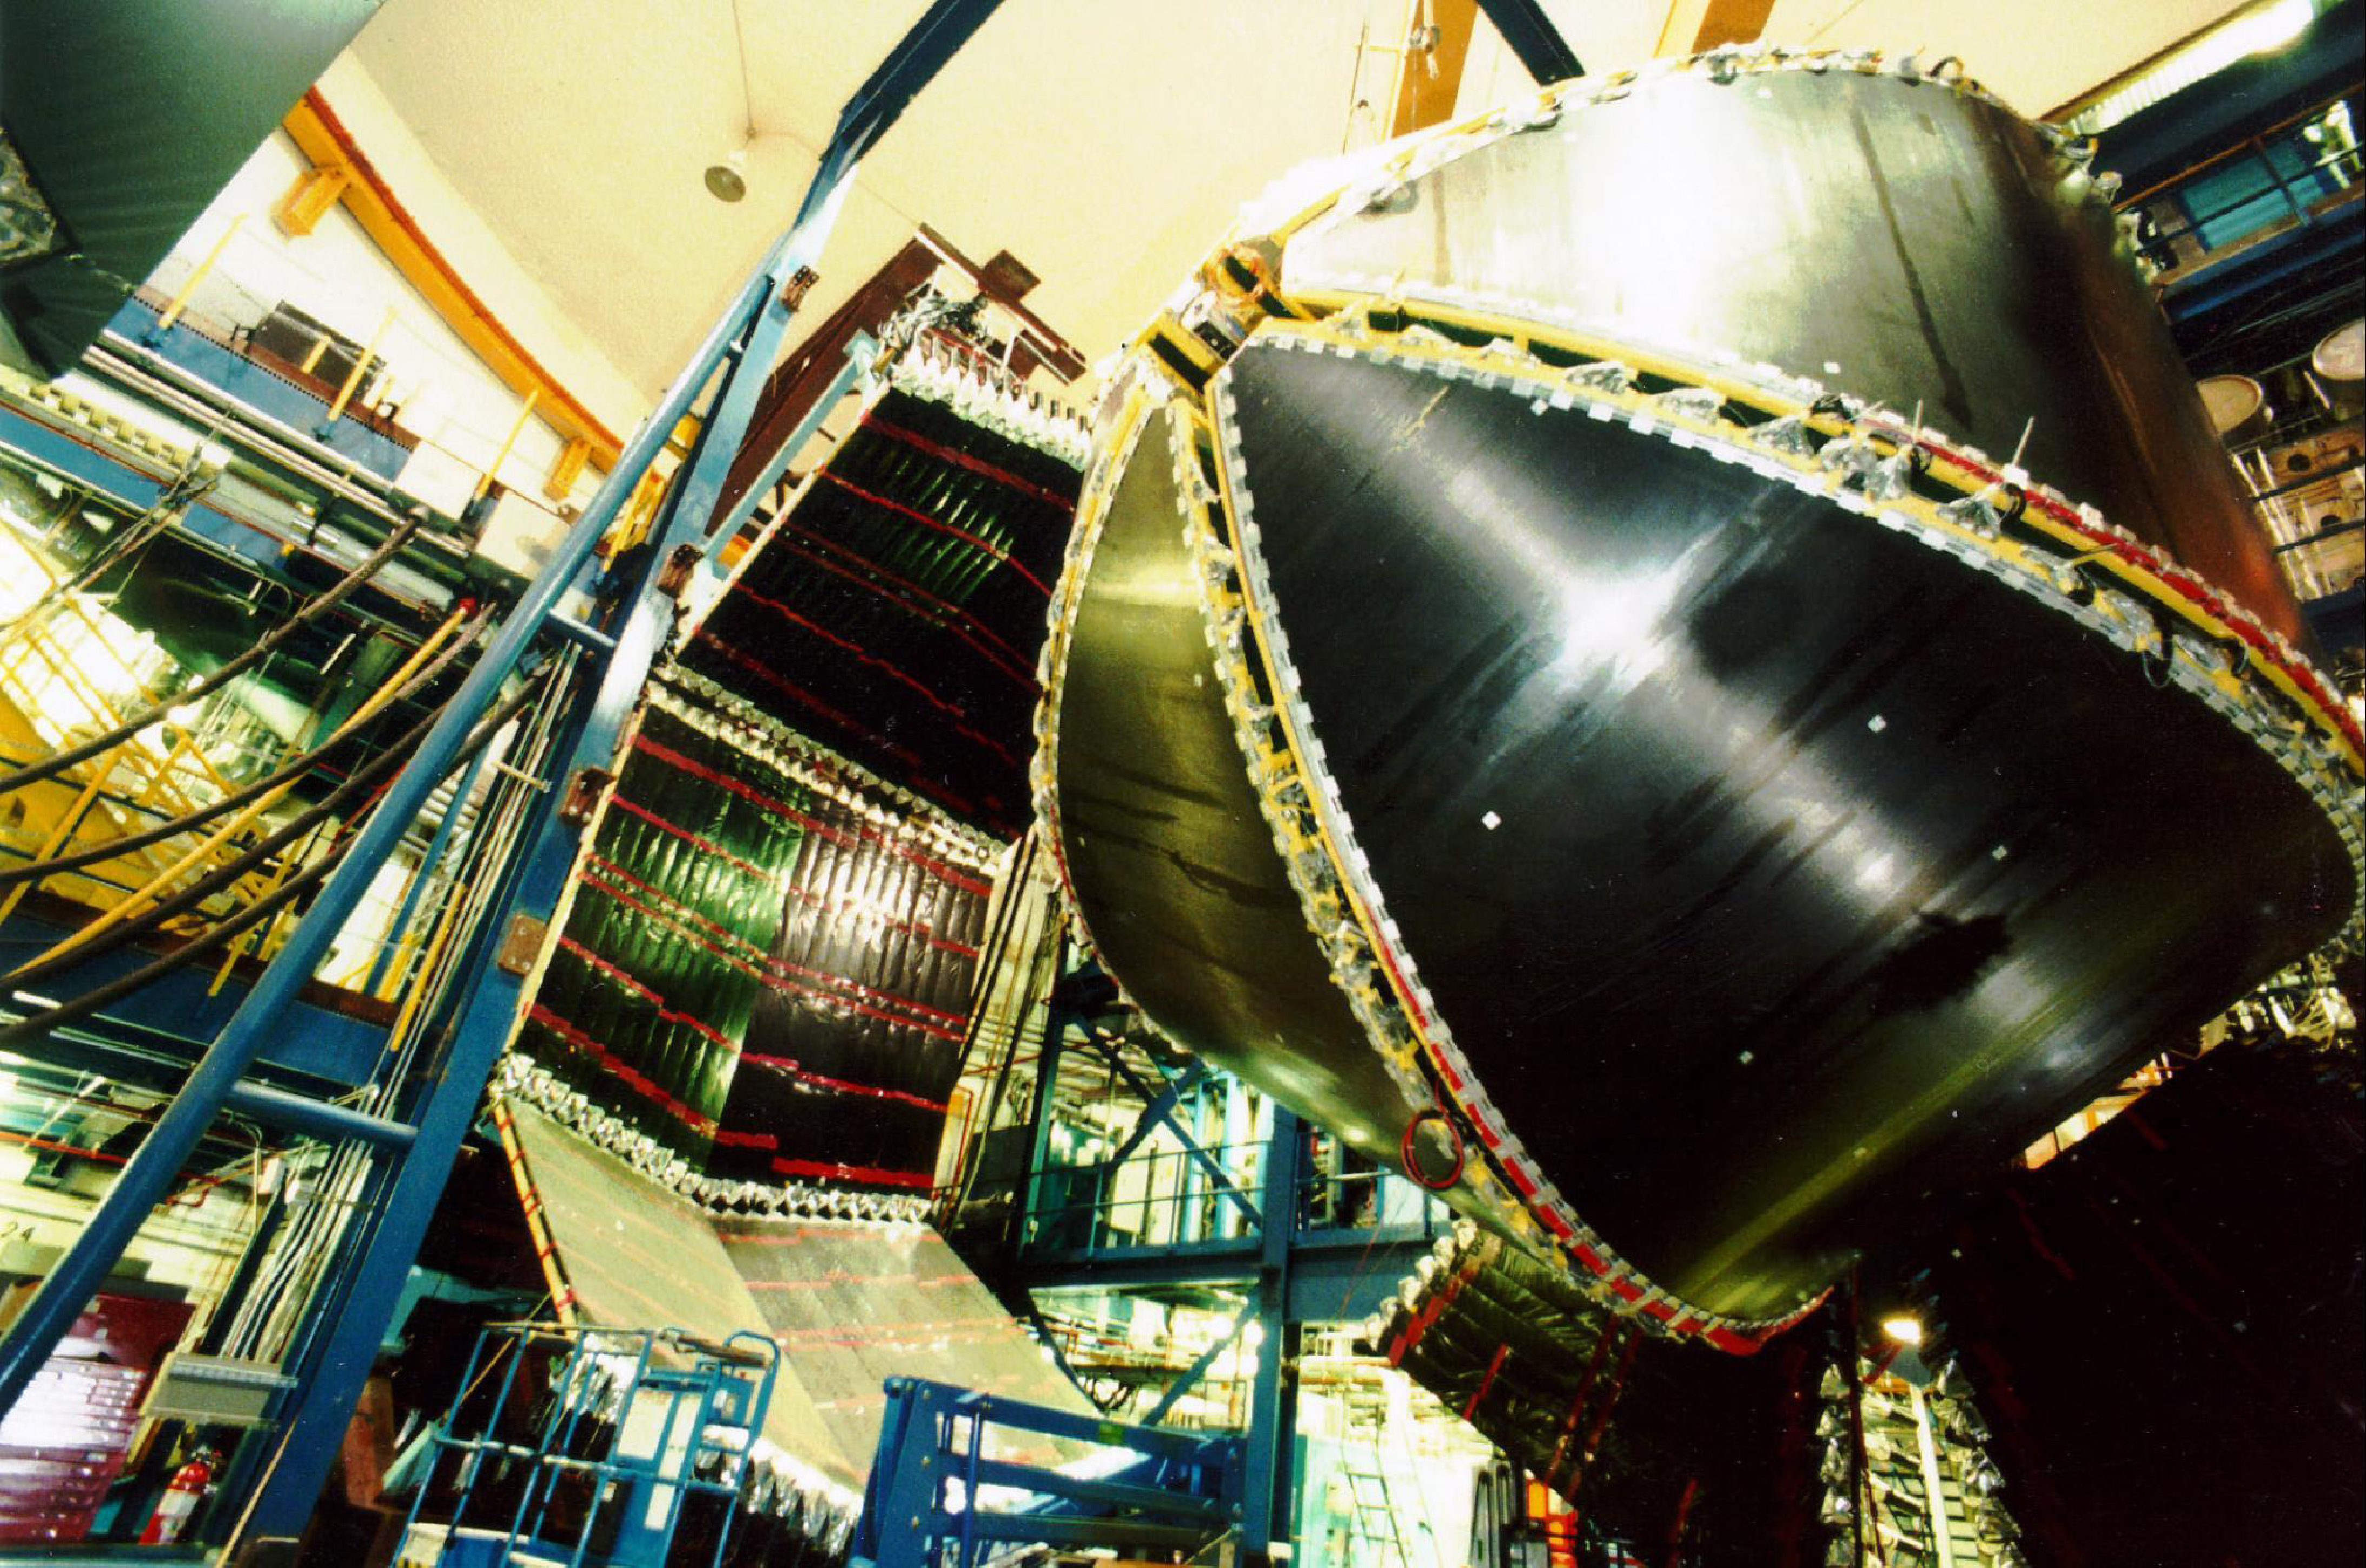
\includegraphics[width=0.8\columnwidth]{\figures/hall-b/clas_detector.pdf}
\caption[\abbr{CLAS} Detector (photograph)]{\label{fig:clas.photo}The \abbr{CLAS} detector during a maintenance period where the time-of-flight ``shell'' (left) was pulled back from the drift-chambers (\abbr{DC}, right). The beam line enters from the lower right on the other side of the \abbr{DC}. The \abbr{TOF} paddles seen are the two center \emph{panels} shown in Fig.~\ref{fig:clas.tof.paddles} for three of the \abbr{CLAS} sectors.}
\end{center}\end{figure}

\begin{figure}\begin{center}
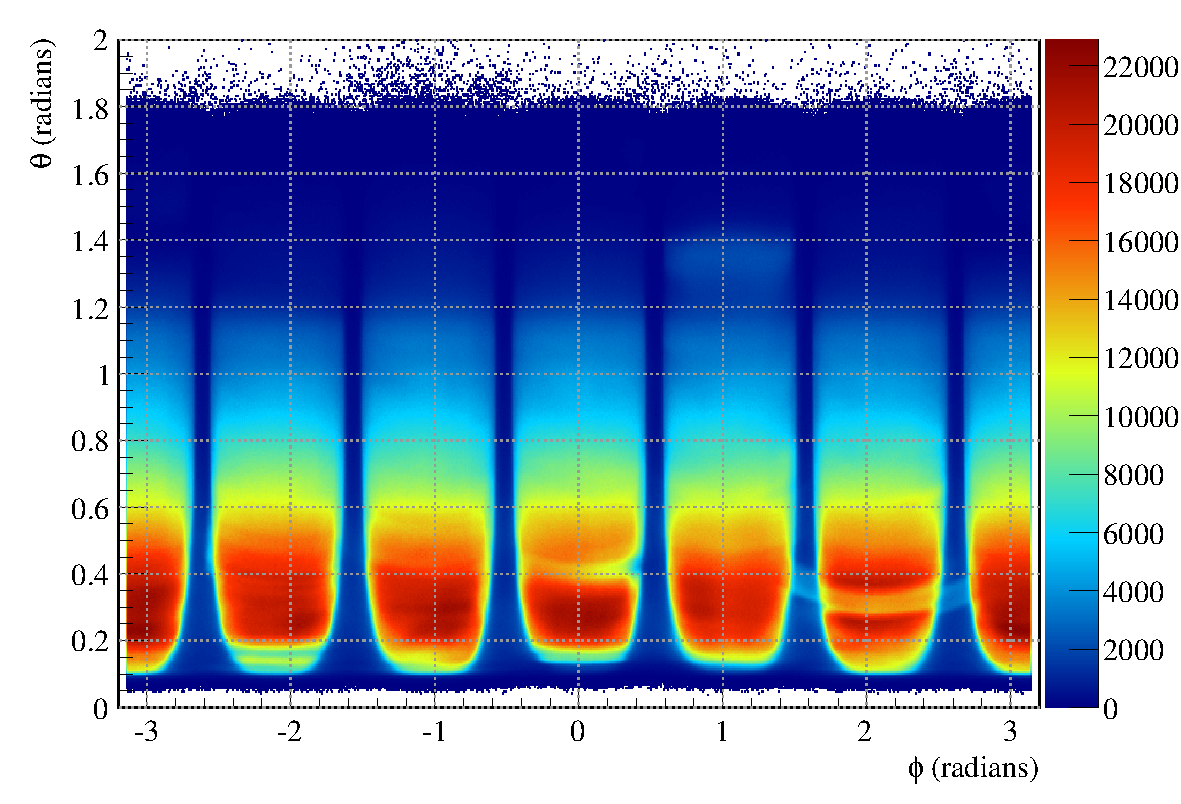
\includegraphics[width=\figwidth]{\figures/reconstruction/coverage_tof.pdf}
\caption[Time-of-Flight Angular Coverage]{\label{fig:clas.tof.coverage}{\coloronline}Angular coverage in the lab frame of the tracks that had an associated time-of-flight hit. This can be interpreted as the total drift-chamber coverage of the \abbr{CLAS} detector.}
\end{center}\end{figure}

\section{Data Aquisition System}\label{sec:clas.daq}

The data acquisition system for the \abbr{CLAS} detector is composed of several layers of electronics. The amplified signals from the various wires and photo-multiplier tubes are received by the \abbr{TDC} and \abbr{ADC} counters. A certain set of these signals are used in the \emph{trigger} to determine if an event of interest has occurred. If it has, then all the signals are sent to the ``event builder'' via \abbr{CAMAC}\label{abbr:camac}\cite{clas} crates and recorded as a single event.

The controlling program makes use of the \abbr{CEBAF} On-line Data Acquisition System (\abbr{CODA}\label{abbr:coda})\cite{clas}. At the time of the \g12 experiment, the \abbr{DAQ} was capable of over 10~kHz. This high rate was due in part to a new field-programmable gate array \abbr{FPGA}\label{abbr:fpga} logic control processor that was integrated into the trigger system for \abbr{CLAS}\cite{clas.trig}.

The input components to the triggering system of \abbr{CLAS} are obtained from the tagger, time-of-flight, start counter, electromagnetic calorimeter and \v{C}erenkov counters. The \abbr{TOF} and \abbr{ST} are used to identify ``prongs,'' or charged tracks, at the trigger level. These composed by a coincidence of any one \abbr{TOF} hit in a given sector with any one \abbr{ST} hit in the same sector. Additionally, a coincidence between the \abbr{EC} and \abbr{CC} above certain thresholds was included as a lepton trigger. The various trigger \emph{bits} used by the system are discussed in Sec.~\ref{sec:data.trig}.

\begin{figure}\begin{center}
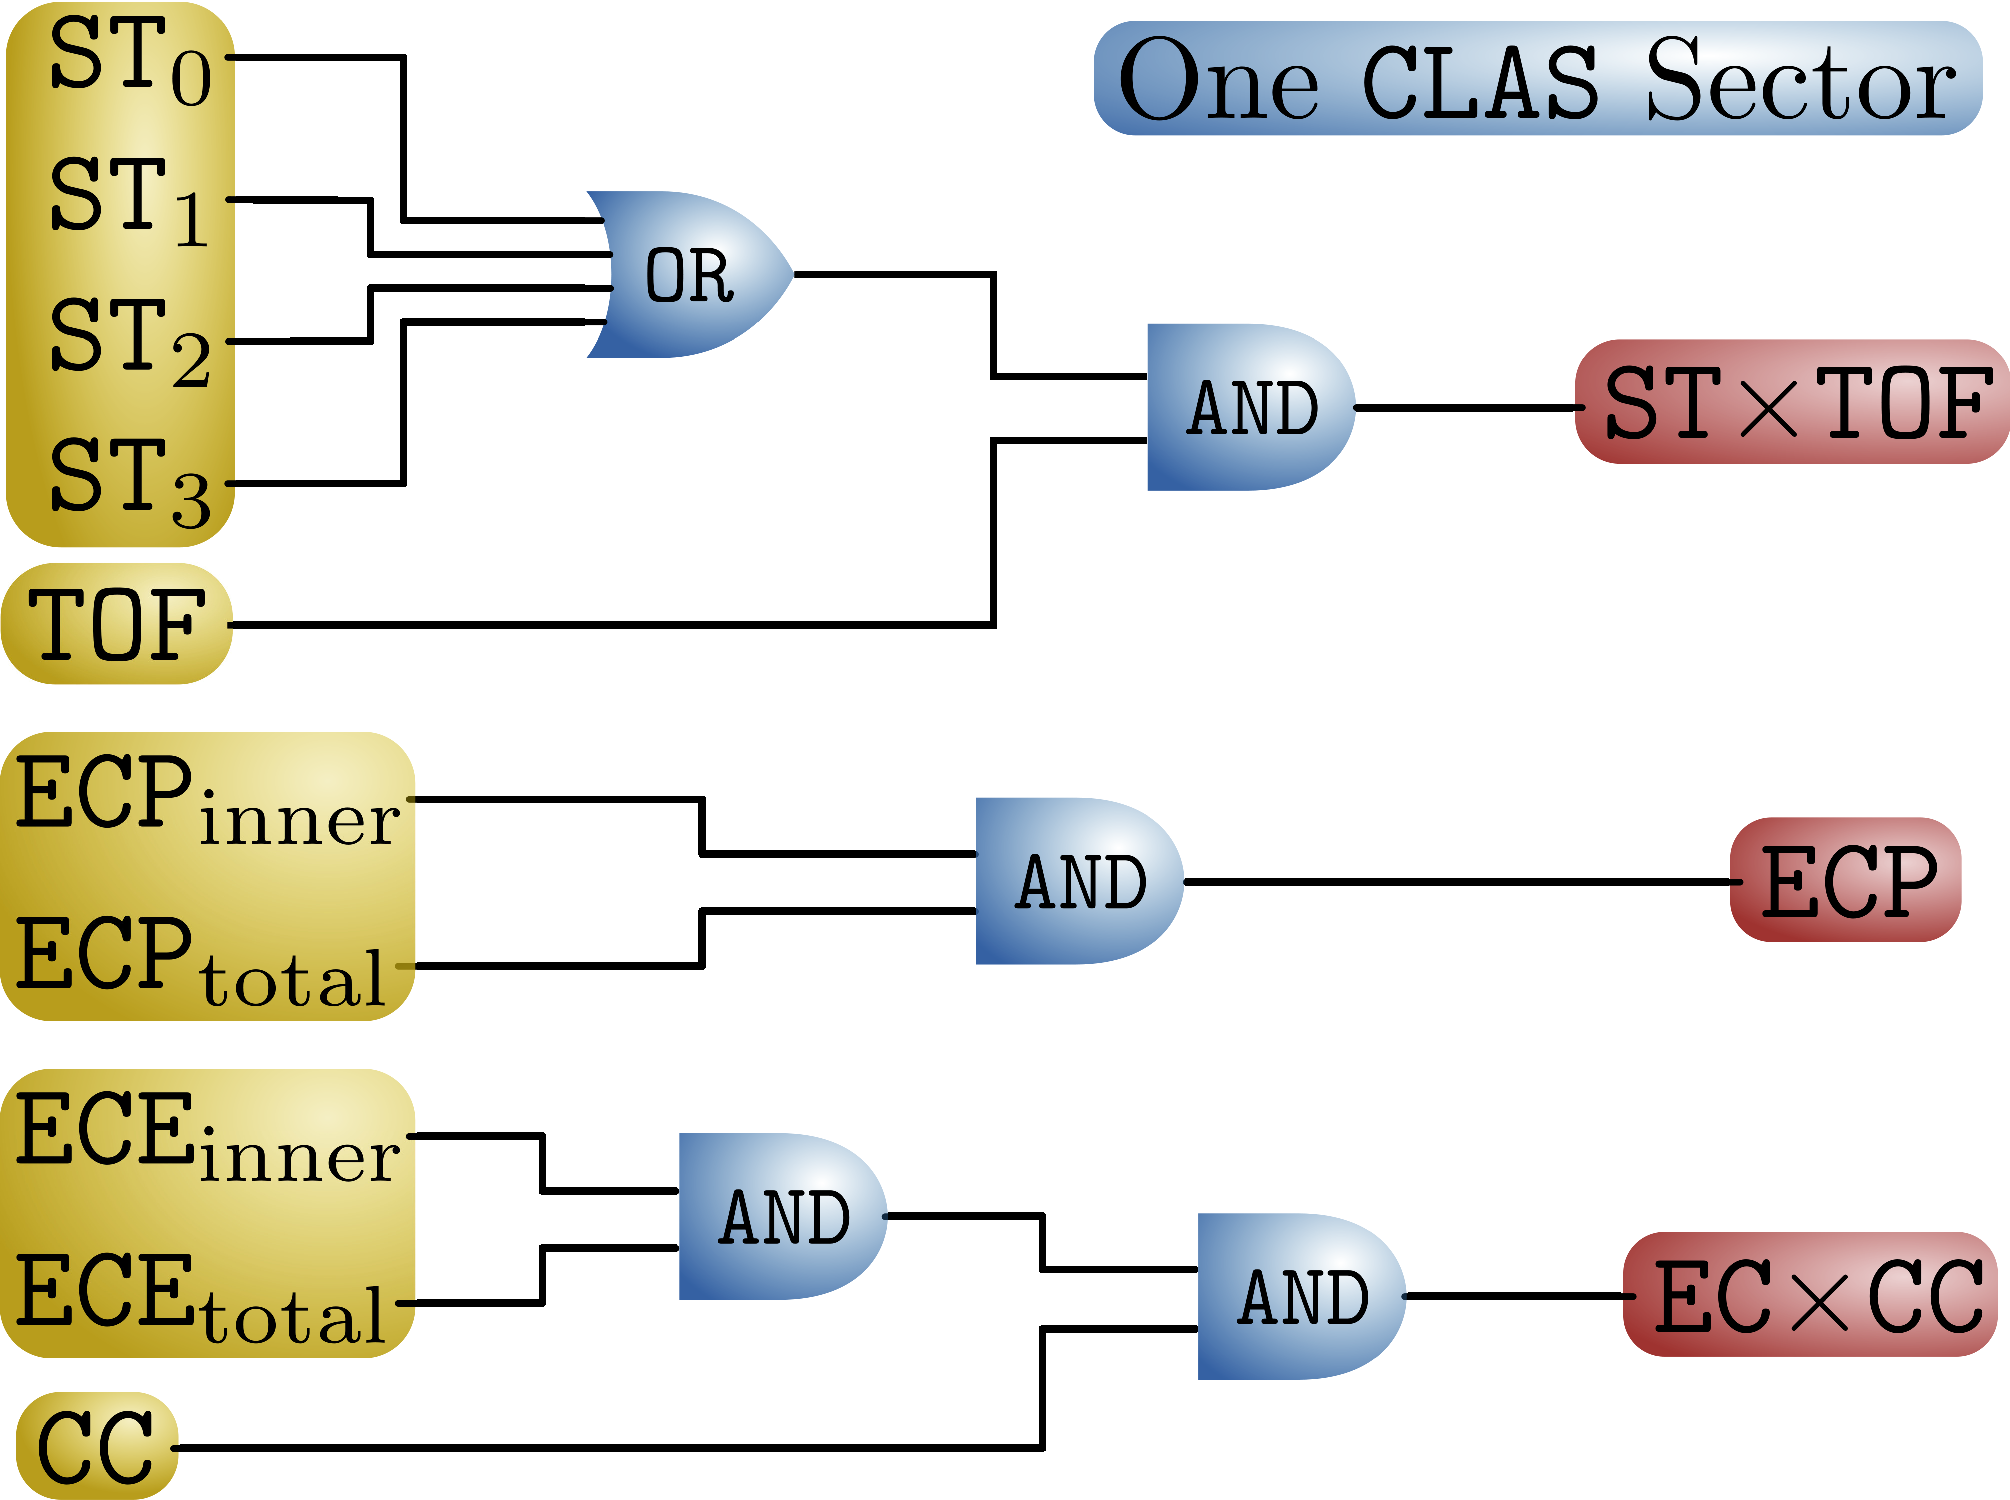
\includegraphics[width=0.8\figwidth]{\figures/hall-b/trigger_sector.pdf}
\caption[Trigger Logic - One Sector]{\label{fig:clas.daq.trigsec}{\coloronline}Trigger logic for one of the six sectors of \abbr{CLAS}. The \abbr{ST$\times$TOF} signal is a coincidence between any of the four start counter \abbr{TDC} signals (numbered from 0 to 3) and any of the 57 \abbr{TOF} \abbr{TDC} signals. The \abbr{ECE}$_\mathrm{inner}$ and \abbr{ECE}$_{\mathrm{total}}$ are the \emph{electron}-threshold \abbr{EC} signals for the energy deposited in the \emph{inner} layer and in \emph{all} layers. These are combined with a \abbr{CC} signal to produce the \abbr{EC$\times$CC} trigger for this sector. The \abbr{ECP} trigger signal is the \emph{photon}-threshold \abbr{EC} signal. These trigger signals are discussed further in Sec.~\ref{sec:data.trig}.}
\end{center}\end{figure}

